\documentclass[twoside]{book}

% Packages required by doxygen
\usepackage{fixltx2e}
\usepackage{calc}
\usepackage{doxygen}
\usepackage[export]{adjustbox} % also loads graphicx
\usepackage{graphicx}
\usepackage[utf8]{inputenc}
\usepackage{makeidx}
\usepackage{multicol}
\usepackage{multirow}
\PassOptionsToPackage{warn}{textcomp}
\usepackage{textcomp}
\usepackage[nointegrals]{wasysym}
\usepackage[table]{xcolor}

% Font selection
\usepackage[T1]{fontenc}
\usepackage[scaled=.90]{helvet}
\usepackage{courier}
\usepackage{amssymb}
\usepackage{sectsty}
\renewcommand{\familydefault}{\sfdefault}
\allsectionsfont{%
  \fontseries{bc}\selectfont%
  \color{darkgray}%
}
\renewcommand{\DoxyLabelFont}{%
  \fontseries{bc}\selectfont%
  \color{darkgray}%
}
\newcommand{\+}{\discretionary{\mbox{\scriptsize$\hookleftarrow$}}{}{}}

% Page & text layout
\usepackage{geometry}
\geometry{%
  a4paper,%
  top=2.5cm,%
  bottom=2.5cm,%
  left_child_=2.5cm,%
  right_child_=2.5cm%
}
\tolerance=750
\hfuzz=15pt
\hbadness=750
\setlength{\emergencystretch}{15pt}
\setlength{\parindent}{0cm}
\setlength{\parskip}{3ex plus 2ex minus 2ex}
\makeatletter
\renewcommand{\paragraph}{%
  \@startsection{paragraph}{4}{0ex}{-1.0ex}{1.0ex}{%
    \normalfont\normalsize\bfseries\SS@parafont%
  }%
}
\renewcommand{\subparagraph}{%
  \@startsection{subparagraph}{5}{0ex}{-1.0ex}{1.0ex}{%
    \normalfont\normalsize\bfseries\SS@subparafont%
  }%
}
\makeatother

% Headers & footers
\usepackage{fancyhdr}
\pagestyle{fancyplain}
\fancyhead[LE]{\fancyplain{}{\bfseries\thepage}}
\fancyhead[CE]{\fancyplain{}{}}
\fancyhead[RE]{\fancyplain{}{\bfseries\leftmark}}
\fancyhead[LO]{\fancyplain{}{\bfseries\rightmark}}
\fancyhead[CO]{\fancyplain{}{}}
\fancyhead[RO]{\fancyplain{}{\bfseries\thepage}}
\fancyfoot[LE]{\fancyplain{}{}}
\fancyfoot[CE]{\fancyplain{}{}}
\fancyfoot[RE]{\fancyplain{}{\bfseries\scriptsize Generated by Doxygen }}
\fancyfoot[LO]{\fancyplain{}{\bfseries\scriptsize Generated by Doxygen }}
\fancyfoot[CO]{\fancyplain{}{}}
\fancyfoot[RO]{\fancyplain{}{}}
\renewcommand{\footrulewidth}{0.4pt}
\renewcommand{\chaptermark}[1]{%
  \markboth{#1}{}%
}
\renewcommand{\sectionmark}[1]{%
  \markright{\thesection\ #1}%
}

% Indices & bibliography
\usepackage{natbib}
\usepackage[titles]{tocloft}
\setcounter{tocdepth}{3}
\setcounter{secnumdepth}{5}
\makeindex

% Custom commands
\newcommand{\clearemptydoublepage}{%
  \newpage{\pagestyle{empty}\cleardoublepage}%
}

\usepackage{caption}
\captionsetup{labelsep=space,justification=centering,font={bf},singlelinecheck=off,skip=4pt,position=top}

%===== C O N T E N T S =====

\begin{document}

% Titlepage & ToC
\pagenumbering{alph}
\begin{titlepage}
\vspace*{7cm}
\begin{center}%
{\Large Huffman \\[1ex]\large 1.\+2 }\\
\vspace*{1cm}
{\large Generated by Doxygen 1.8.13}\\
\end{center}
\end{titlepage}
\clearemptydoublepage
\pagenumbering{roman}
\tableofcontents
\clearemptydoublepage
\pagenumbering{arabic}

%--- Begin generated contents ---
\chapter{Namespace Index}
\section{Namespace List}
Here is a list of all documented namespaces with brief descriptions\+:\begin{DoxyCompactList}
\item\contentsline{section}{\hyperlink{namespacegtest__lite}{gtest\+\_\+lite} \\*Gtest\+\_\+lite\+: a keretrendszer függvényinek és objektumainak névtere }{\pageref{namespacegtest__lite}}{}
\end{DoxyCompactList}

\chapter{Hierarchical Index}
\section{Class Hierarchy}
This inheritance list is sorted roughly, but not completely, alphabetically\+:\begin{DoxyCompactList}
\item \contentsline{section}{\+\_\+\+Is\+\_\+\+Types$<$ F, T $>$}{\pageref{struct___is___types}}{}
\item \contentsline{section}{\+\_\+registry\+\_\+item}{\pageref{struct__registry__item}}{}
\item \contentsline{section}{Bit\+Buffer}{\pageref{class_bit_buffer}}{}
\item \contentsline{section}{call\+\_\+t}{\pageref{structcall__t}}{}
\item \contentsline{section}{Huffman}{\pageref{class_huffman}}{}
\item \contentsline{section}{Letter}{\pageref{class_letter}}{}
\item \contentsline{section}{List$<$ T $>$}{\pageref{class_list}}{}
\item \contentsline{section}{List$<$ char $>$}{\pageref{class_list}}{}
\item \contentsline{section}{Node}{\pageref{class_node}}{}
\begin{DoxyCompactList}
\item \contentsline{section}{End}{\pageref{class_end}}{}
\item \contentsline{section}{Path}{\pageref{class_path}}{}
\end{DoxyCompactList}
\item \contentsline{section}{gtest\+\_\+lite\+:\+:Test}{\pageref{structgtest__lite_1_1_test}}{}
\end{DoxyCompactList}

\chapter{Class Index}
\section{Class List}
Here are the classes, structs, unions and interfaces with brief descriptions\+:\begin{DoxyCompactList}
\item\contentsline{section}{\textbf{ \+\_\+\+Is\+\_\+\+Types$<$ F, T $>$} \\*Segédsablon típuskonverzió futás közbeni ellenőrzésere }{\pageref{struct___is___types}}{}
\item\contentsline{section}{\textbf{ \+\_\+registry\+\_\+item} }{\pageref{struct__registry__item}}{}
\item\contentsline{section}{\textbf{ Bit\+Buffer} }{\pageref{class_bit_buffer}}{}
\item\contentsline{section}{\textbf{ call\+\_\+t} }{\pageref{structcall__t}}{}
\item\contentsline{section}{\textbf{ End} }{\pageref{class_end}}{}
\item\contentsline{section}{\textbf{ Huffman} }{\pageref{class_huffman}}{}
\item\contentsline{section}{\textbf{ Letter} }{\pageref{class_letter}}{}
\item\contentsline{section}{\textbf{ List$<$ T $>$} }{\pageref{class_list}}{}
\item\contentsline{section}{\textbf{ Node} }{\pageref{class_node}}{}
\item\contentsline{section}{\textbf{ Path} }{\pageref{class_path}}{}
\item\contentsline{section}{\textbf{ gtest\+\_\+lite\+::\+Test} }{\pageref{structgtest__lite_1_1_test}}{}
\end{DoxyCompactList}

\chapter{File Index}
\section{File List}
Here is a list of all documented files with brief descriptions\+:\begin{DoxyCompactList}
\item\contentsline{section}{/home/ronaikovacs/\+Prog/\+C++/\+Prog2/hf/huffman\+\_\+1.\+2/{\bfseries bitbuffer.\+h} }{\pageref{bitbuffer_8h}}{}
\item\contentsline{section}{/home/ronaikovacs/\+Prog/\+C++/\+Prog2/hf/huffman\+\_\+1.\+2/\hyperlink{gtest__lite_8h}{gtest\+\_\+lite.\+h} }{\pageref{gtest__lite_8h}}{}
\item\contentsline{section}{/home/ronaikovacs/\+Prog/\+C++/\+Prog2/hf/huffman\+\_\+1.\+2/{\bfseries huffman.\+h} }{\pageref{huffman_8h}}{}
\item\contentsline{section}{/home/ronaikovacs/\+Prog/\+C++/\+Prog2/hf/huffman\+\_\+1.\+2/{\bfseries letter.\+h} }{\pageref{letter_8h}}{}
\item\contentsline{section}{/home/ronaikovacs/\+Prog/\+C++/\+Prog2/hf/huffman\+\_\+1.\+2/{\bfseries list.\+h} }{\pageref{list_8h}}{}
\item\contentsline{section}{/home/ronaikovacs/\+Prog/\+C++/\+Prog2/hf/huffman\+\_\+1.\+2/{\bfseries memtrace.\+h} }{\pageref{memtrace_8h}}{}
\item\contentsline{section}{/home/ronaikovacs/\+Prog/\+C++/\+Prog2/hf/huffman\+\_\+1.\+2/{\bfseries node.\+h} }{\pageref{node_8h}}{}
\end{DoxyCompactList}

\chapter{Namespace Documentation}
\hypertarget{namespacegtest__lite}{}\section{gtest\+\_\+lite Namespace Reference}
\label{namespacegtest__lite}\index{gtest\+\_\+lite@{gtest\+\_\+lite}}


\hyperlink{namespacegtest__lite}{gtest\+\_\+lite}\+: a keretrendszer függvényinek és objektumainak névtere  


\subsection*{Classes}
\begin{DoxyCompactItemize}
\item 
struct \hyperlink{structgtest__lite_1_1_test}{Test}
\end{DoxyCompactItemize}
\subsection*{Functions}
\begin{DoxyCompactItemize}
\item 
\mbox{\Hypertarget{namespacegtest__lite_ab358c162e1cedfc39abf5959417ffc1e}\label{namespacegtest__lite_ab358c162e1cedfc39abf5959417ffc1e}} 
{\footnotesize template$<$typename T $>$ }\\std\+::ostream \& \hyperlink{namespacegtest__lite_ab358c162e1cedfc39abf5959417ffc1e}{E\+X\+P\+E\+C\+T\+\_\+} (T exp, T act, bool($\ast$pred)(T, T), const char $\ast$file, int line, const char $\ast$expr, const char $\ast$lhs=\char`\"{}elvart\char`\"{}, const char $\ast$rhs=\char`\"{}aktual\char`\"{})
\begin{DoxyCompactList}\small\item\em általános sablon a várt értékhez. \end{DoxyCompactList}\item 
\mbox{\Hypertarget{namespacegtest__lite_a8b21cff4e93dcacdd1b4fdb8b6b9c740}\label{namespacegtest__lite_a8b21cff4e93dcacdd1b4fdb8b6b9c740}} 
{\footnotesize template$<$typename T $>$ }\\std\+::ostream \& \hyperlink{namespacegtest__lite_a8b21cff4e93dcacdd1b4fdb8b6b9c740}{E\+X\+P\+E\+C\+T\+\_\+} (T $\ast$exp, T $\ast$act, bool($\ast$pred)(T $\ast$, T $\ast$), const char $\ast$file, int line, const char $\ast$expr, const char $\ast$lhs=\char`\"{}elvart\char`\"{}, const char $\ast$rhs=\char`\"{}aktual\char`\"{})
\begin{DoxyCompactList}\small\item\em pointerre specializált sablon a várt értékhez. \end{DoxyCompactList}\item 
std\+::ostream \& \hyperlink{namespacegtest__lite_aea477921e4c26d2a2806bc3011066270}{E\+X\+P\+E\+C\+T\+S\+TR} (const char $\ast$exp, const char $\ast$act, bool($\ast$pred)(const char $\ast$, const char $\ast$), const char $\ast$file, int line, const char $\ast$expr, const char $\ast$lhs=\char`\"{}elvart\char`\"{}, const char $\ast$rhs=\char`\"{}aktual\char`\"{})
\item 
{\footnotesize template$<$typename T $>$ }\\bool \hyperlink{namespacegtest__lite_aa7762f23094d59c699ec402e1a37640c}{eq} (T a, T b)
\item 
\mbox{\Hypertarget{namespacegtest__lite_a34055f353dabbe4ed9063f1d36af6022}\label{namespacegtest__lite_a34055f353dabbe4ed9063f1d36af6022}} 
bool {\bfseries eqstr} (const char $\ast$a, const char $\ast$b)
\item 
\mbox{\Hypertarget{namespacegtest__lite_a9a1485affebbed604f7cac69f70072dc}\label{namespacegtest__lite_a9a1485affebbed604f7cac69f70072dc}} 
{\footnotesize template$<$typename T $>$ }\\bool {\bfseries ne} (T a, T b)
\item 
\mbox{\Hypertarget{namespacegtest__lite_a0a34b1bb0d55bc0c6a3e878ec2bcd49f}\label{namespacegtest__lite_a0a34b1bb0d55bc0c6a3e878ec2bcd49f}} 
bool {\bfseries nestr} (const char $\ast$a, const char $\ast$b)
\item 
\mbox{\Hypertarget{namespacegtest__lite_a92068d494867b61abeef5942eefac3a3}\label{namespacegtest__lite_a92068d494867b61abeef5942eefac3a3}} 
{\footnotesize template$<$typename T $>$ }\\bool {\bfseries le} (T a, T b)
\item 
\mbox{\Hypertarget{namespacegtest__lite_acfefb55c5d3713c79b659bbd18d9423c}\label{namespacegtest__lite_acfefb55c5d3713c79b659bbd18d9423c}} 
{\footnotesize template$<$typename T $>$ }\\bool {\bfseries lt} (T a, T b)
\item 
\mbox{\Hypertarget{namespacegtest__lite_ae8c2517b99b688c6136d8c7c18551da5}\label{namespacegtest__lite_ae8c2517b99b688c6136d8c7c18551da5}} 
{\footnotesize template$<$typename T $>$ }\\bool {\bfseries ge} (T a, T b)
\item 
\mbox{\Hypertarget{namespacegtest__lite_a2075d101da98f80f569b0737c5185718}\label{namespacegtest__lite_a2075d101da98f80f569b0737c5185718}} 
{\footnotesize template$<$typename T $>$ }\\bool {\bfseries gt} (T a, T b)
\item 
{\footnotesize template$<$typename T $>$ }\\bool \hyperlink{namespacegtest__lite_affbf9748c4e4dec6db137f7c147fee61}{almost\+EQ} (T a, T b)
\end{DoxyCompactItemize}


\subsection{Detailed Description}
\hyperlink{namespacegtest__lite}{gtest\+\_\+lite}\+: a keretrendszer függvényinek és objektumainak névtere 

\subsection{Function Documentation}
\mbox{\Hypertarget{namespacegtest__lite_affbf9748c4e4dec6db137f7c147fee61}\label{namespacegtest__lite_affbf9748c4e4dec6db137f7c147fee61}} 
\index{gtest\+\_\+lite@{gtest\+\_\+lite}!almost\+EQ@{almost\+EQ}}
\index{almost\+EQ@{almost\+EQ}!gtest\+\_\+lite@{gtest\+\_\+lite}}
\subsubsection{\texorpdfstring{almost\+E\+Q()}{almostEQ()}}
{\footnotesize\ttfamily template$<$typename T $>$ \\
bool gtest\+\_\+lite\+::almost\+EQ (\begin{DoxyParamCaption}\item[{T}]{a,  }\item[{T}]{b }\end{DoxyParamCaption})}

Segédsablon valós számok összehasonlításához Nem bombabiztos, de nekünk most jó lesz Elméleti hátér\+: \href{http://www.cygnus-software.com/papers/comparingfloats/comparingfloats.htm}{\tt http\+://www.\+cygnus-\/software.\+com/papers/comparingfloats/comparingfloats.\+htm} \mbox{\Hypertarget{namespacegtest__lite_aa7762f23094d59c699ec402e1a37640c}\label{namespacegtest__lite_aa7762f23094d59c699ec402e1a37640c}} 
\index{gtest\+\_\+lite@{gtest\+\_\+lite}!eq@{eq}}
\index{eq@{eq}!gtest\+\_\+lite@{gtest\+\_\+lite}}
\subsubsection{\texorpdfstring{eq()}{eq()}}
{\footnotesize\ttfamily template$<$typename T $>$ \\
bool gtest\+\_\+lite\+::eq (\begin{DoxyParamCaption}\item[{T}]{a,  }\item[{T}]{b }\end{DoxyParamCaption})}

segéd sablonok a relációkhoz. azért nem S\+TL (algorithm), mert csak a függvény lehet, hogy menjen a deduckció \mbox{\Hypertarget{namespacegtest__lite_aea477921e4c26d2a2806bc3011066270}\label{namespacegtest__lite_aea477921e4c26d2a2806bc3011066270}} 
\index{gtest\+\_\+lite@{gtest\+\_\+lite}!E\+X\+P\+E\+C\+T\+S\+TR@{E\+X\+P\+E\+C\+T\+S\+TR}}
\index{E\+X\+P\+E\+C\+T\+S\+TR@{E\+X\+P\+E\+C\+T\+S\+TR}!gtest\+\_\+lite@{gtest\+\_\+lite}}
\subsubsection{\texorpdfstring{E\+X\+P\+E\+C\+T\+S\+T\+R()}{EXPECTSTR()}}
{\footnotesize\ttfamily std\+::ostream\& gtest\+\_\+lite\+::\+E\+X\+P\+E\+C\+T\+S\+TR (\begin{DoxyParamCaption}\item[{const char $\ast$}]{exp,  }\item[{const char $\ast$}]{act,  }\item[{bool($\ast$)(const char $\ast$, const char $\ast$)}]{pred,  }\item[{const char $\ast$}]{file,  }\item[{int}]{line,  }\item[{const char $\ast$}]{expr,  }\item[{const char $\ast$}]{lhs = {\ttfamily \char`\"{}elvart\char`\"{}},  }\item[{const char $\ast$}]{rhs = {\ttfamily \char`\"{}aktual\char`\"{}} }\end{DoxyParamCaption})\hspace{0.3cm}{\ttfamily [inline]}}

stringek összehasonlításához. azért nem spec. mert a sima E\+Q-\/ra másként kell működnie. 
\chapter{Class Documentation}
\hypertarget{struct___is___types}{}\section{\+\_\+\+Is\+\_\+\+Types$<$ F, T $>$ Struct Template Reference}
\label{struct___is___types}\index{\+\_\+\+Is\+\_\+\+Types$<$ F, T $>$@{\+\_\+\+Is\+\_\+\+Types$<$ F, T $>$}}


Segédsablon típuskonverzió futás közbeni ellenőrzésere.  




{\ttfamily \#include $<$gtest\+\_\+lite.\+h$>$}

\subsection*{Static Public Member Functions}
\begin{DoxyCompactItemize}
\item 
{\footnotesize template$<$typename D $>$ }\\static char(\& \hyperlink{struct___is___types_a56e08a2768c571caab81e9bc47d5acc6}{f} (D))\mbox{[}1\mbox{]}
\item 
{\footnotesize template$<$typename D $>$ }\\static char(\& \hyperlink{struct___is___types_a013da65c5a92e9bd02f5d361c10d376d}{f} (...))\mbox{[}2\mbox{]}
\end{DoxyCompactItemize}
\subsection*{Static Public Attributes}
\begin{DoxyCompactItemize}
\item 
static bool const \hyperlink{struct___is___types_aef853f15f013611d0890cb6fc408ae47}{convertable} = sizeof(\hyperlink{struct___is___types_a56e08a2768c571caab81e9bc47d5acc6}{f}$<$T$>$(F())) == 1
\end{DoxyCompactItemize}


\subsection{Detailed Description}
\subsubsection*{template$<$typename F, typename T$>$\newline
struct \+\_\+\+Is\+\_\+\+Types$<$ F, T $>$}

Segédsablon típuskonverzió futás közbeni ellenőrzésere. 

\subsection{Member Function Documentation}
\mbox{\Hypertarget{struct___is___types_a56e08a2768c571caab81e9bc47d5acc6}\label{struct___is___types_a56e08a2768c571caab81e9bc47d5acc6}} 
\index{\+\_\+\+Is\+\_\+\+Types@{\+\_\+\+Is\+\_\+\+Types}!f@{f}}
\index{f@{f}!\+\_\+\+Is\+\_\+\+Types@{\+\_\+\+Is\+\_\+\+Types}}
\subsubsection{\texorpdfstring{f()}{f()}\hspace{0.1cm}{\footnotesize\ttfamily [1/2]}}
{\footnotesize\ttfamily template$<$typename F , typename T $>$ \\
template$<$typename D $>$ \\
static char(\& \hyperlink{struct___is___types}{\+\_\+\+Is\+\_\+\+Types}$<$ F, T $>$\+::f (\begin{DoxyParamCaption}\item[{D}]{ }\end{DoxyParamCaption}))\mbox{[}1\mbox{]}\hspace{0.3cm}{\ttfamily [static]}}

\mbox{\Hypertarget{struct___is___types_a013da65c5a92e9bd02f5d361c10d376d}\label{struct___is___types_a013da65c5a92e9bd02f5d361c10d376d}} 
\index{\+\_\+\+Is\+\_\+\+Types@{\+\_\+\+Is\+\_\+\+Types}!f@{f}}
\index{f@{f}!\+\_\+\+Is\+\_\+\+Types@{\+\_\+\+Is\+\_\+\+Types}}
\subsubsection{\texorpdfstring{f()}{f()}\hspace{0.1cm}{\footnotesize\ttfamily [2/2]}}
{\footnotesize\ttfamily template$<$typename F , typename T $>$ \\
template$<$typename D $>$ \\
static char(\& \hyperlink{struct___is___types}{\+\_\+\+Is\+\_\+\+Types}$<$ F, T $>$\+::f (\begin{DoxyParamCaption}\item[{}]{... }\end{DoxyParamCaption}))\mbox{[}2\mbox{]}\hspace{0.3cm}{\ttfamily [static]}}



\subsection{Member Data Documentation}
\mbox{\Hypertarget{struct___is___types_aef853f15f013611d0890cb6fc408ae47}\label{struct___is___types_aef853f15f013611d0890cb6fc408ae47}} 
\index{\+\_\+\+Is\+\_\+\+Types@{\+\_\+\+Is\+\_\+\+Types}!convertable@{convertable}}
\index{convertable@{convertable}!\+\_\+\+Is\+\_\+\+Types@{\+\_\+\+Is\+\_\+\+Types}}
\subsubsection{\texorpdfstring{convertable}{convertable}}
{\footnotesize\ttfamily template$<$typename F , typename T $>$ \\
bool const \hyperlink{struct___is___types}{\+\_\+\+Is\+\_\+\+Types}$<$ F, T $>$\+::convertable = sizeof(\hyperlink{struct___is___types_a56e08a2768c571caab81e9bc47d5acc6}{f}$<$T$>$(F())) == 1\hspace{0.3cm}{\ttfamily [static]}}



The documentation for this struct was generated from the following file\+:\begin{DoxyCompactItemize}
\item 
\hyperlink{gtest__lite_8h}{gtest\+\_\+lite.\+h}\end{DoxyCompactItemize}

\section{\+\_\+registry\+\_\+item Struct Reference}
\label{struct__registry__item}\index{\+\_\+registry\+\_\+item@{\+\_\+registry\+\_\+item}}


Collaboration diagram for \+\_\+registry\+\_\+item\+:
\nopagebreak
\begin{figure}[H]
\begin{center}
\leavevmode
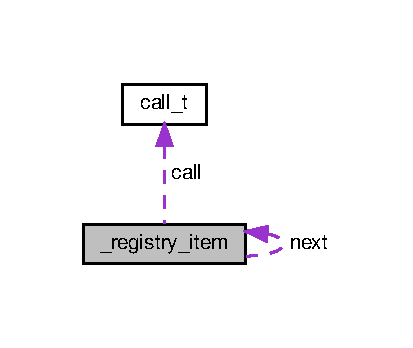
\includegraphics[width=198pt]{struct__registry__item__coll__graph}
\end{center}
\end{figure}
\subsection*{Public Attributes}
\begin{DoxyCompactItemize}
\item 
void $\ast$ \textbf{ p}
\item 
size\+\_\+t \textbf{ size}
\item 
\textbf{ call\+\_\+t} \textbf{ call}
\item 
struct \textbf{ \+\_\+registry\+\_\+item} $\ast$ \textbf{ next}
\end{DoxyCompactItemize}


\subsection{Member data_ Documentation}
\mbox{\label{struct__registry__item_ae5167771e18dc20df38808a4dafa761f}} 
\index{\+\_\+registry\+\_\+item@{\+\_\+registry\+\_\+item}!call@{call}}
\index{call@{call}!\+\_\+registry\+\_\+item@{\+\_\+registry\+\_\+item}}
\subsubsection{call}
{\footnotesize\ttfamily \textbf{ call\+\_\+t} \+\_\+registry\+\_\+item\+::call}

\mbox{\label{struct__registry__item_aa659ff3f2fa74b37e31b0bd3948bbf7f}} 
\index{\+\_\+registry\+\_\+item@{\+\_\+registry\+\_\+item}!next@{next}}
\index{next@{next}!\+\_\+registry\+\_\+item@{\+\_\+registry\+\_\+item}}
\subsubsection{next}
{\footnotesize\ttfamily struct \textbf{ \+\_\+registry\+\_\+item}$\ast$ \+\_\+registry\+\_\+item\+::next}

\mbox{\label{struct__registry__item_a7d2b50523d8801a40d30e17bfab37149}} 
\index{\+\_\+registry\+\_\+item@{\+\_\+registry\+\_\+item}!p@{p}}
\index{p@{p}!\+\_\+registry\+\_\+item@{\+\_\+registry\+\_\+item}}
\subsubsection{p}
{\footnotesize\ttfamily void$\ast$ \+\_\+registry\+\_\+item\+::p}

\mbox{\label{struct__registry__item_a98122f145c9d8ef6b8e34c534307423d}} 
\index{\+\_\+registry\+\_\+item@{\+\_\+registry\+\_\+item}!size@{size}}
\index{size@{size}!\+\_\+registry\+\_\+item@{\+\_\+registry\+\_\+item}}
\subsubsection{size}
{\footnotesize\ttfamily size\+\_\+t \+\_\+registry\+\_\+item\+::size}



The documentation for this struct was generated from the following file\+:\begin{DoxyCompactItemize}
\item 
\textbf{ memtrace.\+cpp}\end{DoxyCompactItemize}

\hypertarget{class_bit_buffer}{}\section{Bit\+Buffer Class Reference}
\label{class_bit_buffer}\index{Bit\+Buffer@{Bit\+Buffer}}


{\ttfamily \#include $<$bitbuffer.\+h$>$}

\subsection*{Public Member Functions}
\begin{DoxyCompactItemize}
\item 
\hyperlink{class_bit_buffer_a9b9c57bd5827f631bb594476323eb861}{Bit\+Buffer} (int size\+\_\+of\+\_\+chunk\+\_\+b=sizeof(char))
\item 
\hyperlink{class_bit_buffer_af78925f3b1d992d934545616c1d00dd2}{Bit\+Buffer} (const \hyperlink{class_bit_buffer}{Bit\+Buffer} \&buffer)
\item 
const \hyperlink{class_list}{List}$<$ char $>$ \& \hyperlink{class_bit_buffer_ad56372e6eb410a195913a0cae28d7006}{data} () const
\item 
char \hyperlink{class_bit_buffer_a3f5383b7d9b27478f614cd8762a266a5}{current\+Chunk} () const
\item 
int \hyperlink{class_bit_buffer_a8c13b651d37586ec5c2d30f45ed89e53}{count} () const
\item 
int \hyperlink{class_bit_buffer_adf758958884467e15cd018190178bf3d}{size\+Of\+Chunk} () const
\item 
int \hyperlink{class_bit_buffer_ad473b6b2aedbb96198d57d5762c5c108}{count\+Of\+Full\+Chunks} () const
\item 
bool \hyperlink{class_bit_buffer_aaec114c48d1b1be84a8178b6b956f3d0}{is\+Empty} ()
\item 
bool \hyperlink{class_bit_buffer_ae70825daafd0a00625fbb6dfb9b83fba}{is\+Open} ()
\item 
{\footnotesize template$<$typename T $>$ }\\void \hyperlink{class_bit_buffer_a1998d0bdd95e025f39e81671f5a20106}{push} (T value\+\_\+bit\+\_\+container, int count\+\_\+of\+\_\+bits)
\item 
char \hyperlink{class_bit_buffer_a8f569dfa9535ac107c84846f22a45221}{pop} ()
\item 
void \hyperlink{class_bit_buffer_a1075aee0daeee83dbe4908c325b6969f}{close} ()
\item 
void \hyperlink{class_bit_buffer_a10df48560dfbdd304a4e05a610379dc8}{leak\+After} (int num\+\_\+of\+\_\+chunks)
\item 
int \hyperlink{class_bit_buffer_a28c31e06cd23a8ab3f7276bbb2c64b39}{leak\+After} () const
\item 
void \hyperlink{class_bit_buffer_a56d1e27a00a27e1ac95f2e03255081eb}{leak} (std\+::ostream \&stream\+\_\+out)
\item 
void \hyperlink{class_bit_buffer_a91b2bfeb34d3e2d01fd23f417928f261}{fill} (std\+::istream \&stream\+\_\+in)
\item 
bool \hyperlink{class_bit_buffer_a50d13861a778aff828e42e4f32371726}{bit} ()
\end{DoxyCompactItemize}


\subsection{Detailed Description}
This class can hold bits. Useful when size of values to be stored is not constant. 

\subsection{Constructor \& Destructor Documentation}
\mbox{\Hypertarget{class_bit_buffer_a9b9c57bd5827f631bb594476323eb861}\label{class_bit_buffer_a9b9c57bd5827f631bb594476323eb861}} 
\index{Bit\+Buffer@{Bit\+Buffer}!Bit\+Buffer@{Bit\+Buffer}}
\index{Bit\+Buffer@{Bit\+Buffer}!Bit\+Buffer@{Bit\+Buffer}}
\subsubsection{\texorpdfstring{Bit\+Buffer()}{BitBuffer()}\hspace{0.1cm}{\footnotesize\ttfamily [1/2]}}
{\footnotesize\ttfamily Bit\+Buffer\+::\+Bit\+Buffer (\begin{DoxyParamCaption}\item[{int}]{size\+\_\+of\+\_\+chunk\+\_\+b = {\ttfamily sizeof(char)} }\end{DoxyParamCaption})\hspace{0.3cm}{\ttfamily [explicit]}}

Buffer 
\begin{DoxyParams}{Parameters}
{\em size\+\_\+of\+\_\+chunk\+\_\+b} & Number of bits each chunk can store (character\textquotesingle{}s size by default) \\
\hline
\end{DoxyParams}
\mbox{\Hypertarget{class_bit_buffer_af78925f3b1d992d934545616c1d00dd2}\label{class_bit_buffer_af78925f3b1d992d934545616c1d00dd2}} 
\index{Bit\+Buffer@{Bit\+Buffer}!Bit\+Buffer@{Bit\+Buffer}}
\index{Bit\+Buffer@{Bit\+Buffer}!Bit\+Buffer@{Bit\+Buffer}}
\subsubsection{\texorpdfstring{Bit\+Buffer()}{BitBuffer()}\hspace{0.1cm}{\footnotesize\ttfamily [2/2]}}
{\footnotesize\ttfamily Bit\+Buffer\+::\+Bit\+Buffer (\begin{DoxyParamCaption}\item[{const \hyperlink{class_bit_buffer}{Bit\+Buffer} \&}]{buffer }\end{DoxyParamCaption})}

Buffer 
\begin{DoxyParams}{Parameters}
{\em buffer} & A buffer to be copied (resulting Buffer is editable) \\
\hline
\end{DoxyParams}


\subsection{Member Function Documentation}
\mbox{\Hypertarget{class_bit_buffer_a50d13861a778aff828e42e4f32371726}\label{class_bit_buffer_a50d13861a778aff828e42e4f32371726}} 
\index{Bit\+Buffer@{Bit\+Buffer}!bit@{bit}}
\index{bit@{bit}!Bit\+Buffer@{Bit\+Buffer}}
\subsubsection{\texorpdfstring{bit()}{bit()}}
{\footnotesize\ttfamily bool Bit\+Buffer\+::bit (\begin{DoxyParamCaption}{ }\end{DoxyParamCaption})}

Returning the first (not yet returned) bit from buffer \begin{DoxyReturn}{Returns}
True = 1, False = 0 bit 
\end{DoxyReturn}
\mbox{\Hypertarget{class_bit_buffer_a1075aee0daeee83dbe4908c325b6969f}\label{class_bit_buffer_a1075aee0daeee83dbe4908c325b6969f}} 
\index{Bit\+Buffer@{Bit\+Buffer}!close@{close}}
\index{close@{close}!Bit\+Buffer@{Bit\+Buffer}}
\subsubsection{\texorpdfstring{close()}{close()}}
{\footnotesize\ttfamily void Bit\+Buffer\+::close (\begin{DoxyParamCaption}{ }\end{DoxyParamCaption})}

Closing the buffer This makes sure that all data\+\_\+ is stored properly; using \hyperlink{class_bit_buffer_a1998d0bdd95e025f39e81671f5a20106}{push()} will not be allowed anymore. \mbox{\Hypertarget{class_bit_buffer_a8c13b651d37586ec5c2d30f45ed89e53}\label{class_bit_buffer_a8c13b651d37586ec5c2d30f45ed89e53}} 
\index{Bit\+Buffer@{Bit\+Buffer}!count@{count}}
\index{count@{count}!Bit\+Buffer@{Bit\+Buffer}}
\subsubsection{\texorpdfstring{count()}{count()}}
{\footnotesize\ttfamily int Bit\+Buffer\+::count (\begin{DoxyParamCaption}{ }\end{DoxyParamCaption}) const\hspace{0.3cm}{\ttfamily [inline]}}

\begin{DoxyReturn}{Returns}
Count of valuable bits in \hyperlink{class_bit_buffer_a3f5383b7d9b27478f614cd8762a266a5}{current\+Chunk()} 
\end{DoxyReturn}
\mbox{\Hypertarget{class_bit_buffer_ad473b6b2aedbb96198d57d5762c5c108}\label{class_bit_buffer_ad473b6b2aedbb96198d57d5762c5c108}} 
\index{Bit\+Buffer@{Bit\+Buffer}!count\+Of\+Full\+Chunks@{count\+Of\+Full\+Chunks}}
\index{count\+Of\+Full\+Chunks@{count\+Of\+Full\+Chunks}!Bit\+Buffer@{Bit\+Buffer}}
\subsubsection{\texorpdfstring{count\+Of\+Full\+Chunks()}{countOfFullChunks()}}
{\footnotesize\ttfamily int Bit\+Buffer\+::count\+Of\+Full\+Chunks (\begin{DoxyParamCaption}{ }\end{DoxyParamCaption}) const\hspace{0.3cm}{\ttfamily [inline]}}

\begin{DoxyReturn}{Returns}
Number of full chunks. 
\end{DoxyReturn}
\mbox{\Hypertarget{class_bit_buffer_a3f5383b7d9b27478f614cd8762a266a5}\label{class_bit_buffer_a3f5383b7d9b27478f614cd8762a266a5}} 
\index{Bit\+Buffer@{Bit\+Buffer}!current\+Chunk@{current\+Chunk}}
\index{current\+Chunk@{current\+Chunk}!Bit\+Buffer@{Bit\+Buffer}}
\subsubsection{\texorpdfstring{current\+Chunk()}{currentChunk()}}
{\footnotesize\ttfamily char Bit\+Buffer\+::current\+Chunk (\begin{DoxyParamCaption}{ }\end{DoxyParamCaption}) const\hspace{0.3cm}{\ttfamily [inline]}}

\begin{DoxyReturn}{Returns}
Last (not yet full) chunk of data\+\_\+. The last \hyperlink{class_bit_buffer_a8c13b651d37586ec5c2d30f45ed89e53}{count()} bits are values. 
\end{DoxyReturn}
\mbox{\Hypertarget{class_bit_buffer_ad56372e6eb410a195913a0cae28d7006}\label{class_bit_buffer_ad56372e6eb410a195913a0cae28d7006}} 
\index{Bit\+Buffer@{Bit\+Buffer}!data@{data}}
\index{data@{data}!Bit\+Buffer@{Bit\+Buffer}}
\subsubsection{\texorpdfstring{data()}{data()}}
{\footnotesize\ttfamily const \hyperlink{class_list}{List}$<$char$>$\& Bit\+Buffer\+::data (\begin{DoxyParamCaption}{ }\end{DoxyParamCaption}) const\hspace{0.3cm}{\ttfamily [inline]}}

\begin{DoxyReturn}{Returns}
data\+\_\+ stored so far 
\end{DoxyReturn}
\mbox{\Hypertarget{class_bit_buffer_a91b2bfeb34d3e2d01fd23f417928f261}\label{class_bit_buffer_a91b2bfeb34d3e2d01fd23f417928f261}} 
\index{Bit\+Buffer@{Bit\+Buffer}!fill@{fill}}
\index{fill@{fill}!Bit\+Buffer@{Bit\+Buffer}}
\subsubsection{\texorpdfstring{fill()}{fill()}}
{\footnotesize\ttfamily void Bit\+Buffer\+::fill (\begin{DoxyParamCaption}\item[{std\+::istream \&}]{stream\+\_\+in }\end{DoxyParamCaption})}

Getting some data\+\_\+ from file After call, at least 1 full character will be stream\+\_\+in the buffer. \mbox{\Hypertarget{class_bit_buffer_aaec114c48d1b1be84a8178b6b956f3d0}\label{class_bit_buffer_aaec114c48d1b1be84a8178b6b956f3d0}} 
\index{Bit\+Buffer@{Bit\+Buffer}!is\+Empty@{is\+Empty}}
\index{is\+Empty@{is\+Empty}!Bit\+Buffer@{Bit\+Buffer}}
\subsubsection{\texorpdfstring{is\+Empty()}{isEmpty()}}
{\footnotesize\ttfamily bool Bit\+Buffer\+::is\+Empty (\begin{DoxyParamCaption}{ }\end{DoxyParamCaption})\hspace{0.3cm}{\ttfamily [inline]}}

\begin{DoxyReturn}{Returns}
true, if there is no \hyperlink{class_bit_buffer_a8f569dfa9535ac107c84846f22a45221}{pop()}-\/able data\+\_\+ in the buffer 
\end{DoxyReturn}
\mbox{\Hypertarget{class_bit_buffer_ae70825daafd0a00625fbb6dfb9b83fba}\label{class_bit_buffer_ae70825daafd0a00625fbb6dfb9b83fba}} 
\index{Bit\+Buffer@{Bit\+Buffer}!is\+Open@{is\+Open}}
\index{is\+Open@{is\+Open}!Bit\+Buffer@{Bit\+Buffer}}
\subsubsection{\texorpdfstring{is\+Open()}{isOpen()}}
{\footnotesize\ttfamily bool Bit\+Buffer\+::is\+Open (\begin{DoxyParamCaption}{ }\end{DoxyParamCaption})\hspace{0.3cm}{\ttfamily [inline]}}

\begin{DoxyReturn}{Returns}
Whether buffer is open (bits can be \hyperlink{class_bit_buffer_a1998d0bdd95e025f39e81671f5a20106}{push()}-\/ed) 
\end{DoxyReturn}
\mbox{\Hypertarget{class_bit_buffer_a56d1e27a00a27e1ac95f2e03255081eb}\label{class_bit_buffer_a56d1e27a00a27e1ac95f2e03255081eb}} 
\index{Bit\+Buffer@{Bit\+Buffer}!leak@{leak}}
\index{leak@{leak}!Bit\+Buffer@{Bit\+Buffer}}
\subsubsection{\texorpdfstring{leak()}{leak()}}
{\footnotesize\ttfamily void Bit\+Buffer\+::leak (\begin{DoxyParamCaption}\item[{std\+::ostream \&}]{stream\+\_\+out }\end{DoxyParamCaption})}

Leaking data\+\_\+ to a file When there\textquotesingle{}are more chunks than the leak-\/size, those all go to the file \mbox{\Hypertarget{class_bit_buffer_a10df48560dfbdd304a4e05a610379dc8}\label{class_bit_buffer_a10df48560dfbdd304a4e05a610379dc8}} 
\index{Bit\+Buffer@{Bit\+Buffer}!leak\+After@{leak\+After}}
\index{leak\+After@{leak\+After}!Bit\+Buffer@{Bit\+Buffer}}
\subsubsection{\texorpdfstring{leak\+After()}{leakAfter()}\hspace{0.1cm}{\footnotesize\ttfamily [1/2]}}
{\footnotesize\ttfamily void Bit\+Buffer\+::leak\+After (\begin{DoxyParamCaption}\item[{int}]{num\+\_\+of\+\_\+chunks }\end{DoxyParamCaption})}

Setting the leak-\/size \mbox{\Hypertarget{class_bit_buffer_a28c31e06cd23a8ab3f7276bbb2c64b39}\label{class_bit_buffer_a28c31e06cd23a8ab3f7276bbb2c64b39}} 
\index{Bit\+Buffer@{Bit\+Buffer}!leak\+After@{leak\+After}}
\index{leak\+After@{leak\+After}!Bit\+Buffer@{Bit\+Buffer}}
\subsubsection{\texorpdfstring{leak\+After()}{leakAfter()}\hspace{0.1cm}{\footnotesize\ttfamily [2/2]}}
{\footnotesize\ttfamily int Bit\+Buffer\+::leak\+After (\begin{DoxyParamCaption}{ }\end{DoxyParamCaption}) const}

Get leak-\/size \mbox{\Hypertarget{class_bit_buffer_a8f569dfa9535ac107c84846f22a45221}\label{class_bit_buffer_a8f569dfa9535ac107c84846f22a45221}} 
\index{Bit\+Buffer@{Bit\+Buffer}!pop@{pop}}
\index{pop@{pop}!Bit\+Buffer@{Bit\+Buffer}}
\subsubsection{\texorpdfstring{pop()}{pop()}}
{\footnotesize\ttfamily char Bit\+Buffer\+::pop (\begin{DoxyParamCaption}{ }\end{DoxyParamCaption})}

Returning the first chunk The returned chunk will be removed from buffer. \begin{DoxyReturn}{Returns}
The first chunk 
\end{DoxyReturn}
\mbox{\Hypertarget{class_bit_buffer_a1998d0bdd95e025f39e81671f5a20106}\label{class_bit_buffer_a1998d0bdd95e025f39e81671f5a20106}} 
\index{Bit\+Buffer@{Bit\+Buffer}!push@{push}}
\index{push@{push}!Bit\+Buffer@{Bit\+Buffer}}
\subsubsection{\texorpdfstring{push()}{push()}}
{\footnotesize\ttfamily template$<$typename T $>$ \\
void Bit\+Buffer\+::push (\begin{DoxyParamCaption}\item[{T}]{value\+\_\+bit\+\_\+container,  }\item[{int}]{count\+\_\+of\+\_\+bits }\end{DoxyParamCaption})\hspace{0.3cm}{\ttfamily [inline]}}

Adding bits to the buffer Pushes the given bits into the buffer (current\+\_\+chunk\+\_\+). 
\begin{DoxyParams}{Parameters}
{\em value\+\_\+bit\+\_\+container} & It contains the value-\/bits (fitted to the right\+\_\+child\+\_\+=L\+SB). \\
\hline
{\em count\+\_\+of\+\_\+bits} & Number of significant bits. \\
\hline
\end{DoxyParams}
\mbox{\Hypertarget{class_bit_buffer_adf758958884467e15cd018190178bf3d}\label{class_bit_buffer_adf758958884467e15cd018190178bf3d}} 
\index{Bit\+Buffer@{Bit\+Buffer}!size\+Of\+Chunk@{size\+Of\+Chunk}}
\index{size\+Of\+Chunk@{size\+Of\+Chunk}!Bit\+Buffer@{Bit\+Buffer}}
\subsubsection{\texorpdfstring{size\+Of\+Chunk()}{sizeOfChunk()}}
{\footnotesize\ttfamily int Bit\+Buffer\+::size\+Of\+Chunk (\begin{DoxyParamCaption}{ }\end{DoxyParamCaption}) const\hspace{0.3cm}{\ttfamily [inline]}}

\begin{DoxyReturn}{Returns}
Count of bits in each chunk. 
\end{DoxyReturn}


The documentation for this class was generated from the following files\+:\begin{DoxyCompactItemize}
\item 
\hyperlink{bitbuffer_8h}{bitbuffer.\+h}\item 
\hyperlink{bitbuffer_8cpp}{bitbuffer.\+cpp}\end{DoxyCompactItemize}

\hypertarget{structcall__t}{}\section{call\+\_\+t Struct Reference}
\label{structcall__t}\index{call\+\_\+t@{call\+\_\+t}}
\subsection*{Public Attributes}
\begin{DoxyCompactItemize}
\item 
\mbox{\Hypertarget{structcall__t_a59d4e803f2e254dc5ceeb9c1bfcc9355}\label{structcall__t_a59d4e803f2e254dc5ceeb9c1bfcc9355}} 
int {\bfseries f}
\item 
\mbox{\Hypertarget{structcall__t_aaa4f0e556289bbf4da414897b10e0916}\label{structcall__t_aaa4f0e556289bbf4da414897b10e0916}} 
int {\bfseries line}
\item 
\mbox{\Hypertarget{structcall__t_a24e185188a17e272396e118640672aba}\label{structcall__t_a24e185188a17e272396e118640672aba}} 
char $\ast$ {\bfseries par\+\_\+txt}
\item 
\mbox{\Hypertarget{structcall__t_a97629ec51d024396221fe7d48c84859a}\label{structcall__t_a97629ec51d024396221fe7d48c84859a}} 
char $\ast$ {\bfseries file}
\end{DoxyCompactItemize}


The documentation for this struct was generated from the following file\+:\begin{DoxyCompactItemize}
\item 
/home/ronaikovacs/\+Prog/\+C++/\+Prog2/hf/huffman\+\_\+1.\+2/memtrace.\+cpp\end{DoxyCompactItemize}

\hypertarget{class_end}{}\section{End Class Reference}
\label{class_end}\index{End@{End}}


{\ttfamily \#include $<$node.\+h$>$}



Inherits \hyperlink{class_node}{Node}.

\subsection*{Public Member Functions}
\begin{DoxyCompactItemize}
\item 
\hyperlink{class_end_aec010332b2484030781dff4ab47156ce}{End} (\hyperlink{class_letter}{Letter} \&\hyperlink{class_end_a8528f92e9da9ac41a938c559b50eb174}{letter}, long frequency)
\item 
\hyperlink{class_end_a9cdb20f0a78b188e13de7c4afc1a0bf4}{End} (const \hyperlink{class_end}{End} \&end)
\item 
\hyperlink{class_end_acd25fa8f481c50f5b8eaff4af1159942}{End} ()
\item 
\hyperlink{class_letter}{Letter} \& \hyperlink{class_end_a8528f92e9da9ac41a938c559b50eb174}{letter} ()
\item 
\hyperlink{class_node}{Node} $\ast$ \hyperlink{class_end_a812df7f23fffdb2274ca2003ebd8e884}{left} () const
\item 
\hyperlink{class_node}{Node} $\ast$ \hyperlink{class_end_ac8e651d50ce2b99256be11aa9b89ded4}{right} () const
\item 
bool \hyperlink{class_end_a0be5ea8a94107bb8c3a0a2eb19d8188c}{operator==} (\hyperlink{class_end}{End} \&end)
\item 
bool \hyperlink{class_end_a0b3d32d1f08031447f6facf17ee17dff}{operator==} (char ch)
\item 
void \hyperlink{class_end_aa1acae6e027fc01427b07afe58f44f09}{operator++} (int)
\end{DoxyCompactItemize}
\subsection*{Additional Inherited Members}


\subsection{Detailed Description}
Represent a \hyperlink{class_node}{Node} of a binary (\hyperlink{class_huffman}{Huffman}) tree, which IS a leaf 

\subsection{Constructor \& Destructor Documentation}
\mbox{\Hypertarget{class_end_aec010332b2484030781dff4ab47156ce}\label{class_end_aec010332b2484030781dff4ab47156ce}} 
\index{End@{End}!End@{End}}
\index{End@{End}!End@{End}}
\subsubsection{\texorpdfstring{End()}{End()}\hspace{0.1cm}{\footnotesize\ttfamily [1/3]}}
{\footnotesize\ttfamily End\+::\+End (\begin{DoxyParamCaption}\item[{\hyperlink{class_letter}{Letter} \&}]{letter,  }\item[{long}]{frequency }\end{DoxyParamCaption})}

Constructor 
\begin{DoxyParams}{Parameters}
{\em letter} & The represented \hyperlink{class_letter}{Letter} \\
\hline
{\em frequency} & Frequency of the letter in input \\
\hline
\end{DoxyParams}
\mbox{\Hypertarget{class_end_a9cdb20f0a78b188e13de7c4afc1a0bf4}\label{class_end_a9cdb20f0a78b188e13de7c4afc1a0bf4}} 
\index{End@{End}!End@{End}}
\index{End@{End}!End@{End}}
\subsubsection{\texorpdfstring{End()}{End()}\hspace{0.1cm}{\footnotesize\ttfamily [2/3]}}
{\footnotesize\ttfamily End\+::\+End (\begin{DoxyParamCaption}\item[{const \hyperlink{class_end}{End} \&}]{end }\end{DoxyParamCaption})}

Copy constructor \mbox{\Hypertarget{class_end_acd25fa8f481c50f5b8eaff4af1159942}\label{class_end_acd25fa8f481c50f5b8eaff4af1159942}} 
\index{End@{End}!End@{End}}
\index{End@{End}!End@{End}}
\subsubsection{\texorpdfstring{End()}{End()}\hspace{0.1cm}{\footnotesize\ttfamily [3/3]}}
{\footnotesize\ttfamily End\+::\+End (\begin{DoxyParamCaption}{ }\end{DoxyParamCaption})}

is\+Empty end-\/node; useful for arrays 

\subsection{Member Function Documentation}
\mbox{\Hypertarget{class_end_a812df7f23fffdb2274ca2003ebd8e884}\label{class_end_a812df7f23fffdb2274ca2003ebd8e884}} 
\index{End@{End}!left@{left}}
\index{left@{left}!End@{End}}
\subsubsection{\texorpdfstring{left()}{left()}}
{\footnotesize\ttfamily \hyperlink{class_node}{Node} $\ast$ End\+::left (\begin{DoxyParamCaption}{ }\end{DoxyParamCaption}) const}

left\+\_\+child\+\_\+ child \mbox{\Hypertarget{class_end_a8528f92e9da9ac41a938c559b50eb174}\label{class_end_a8528f92e9da9ac41a938c559b50eb174}} 
\index{End@{End}!letter@{letter}}
\index{letter@{letter}!End@{End}}
\subsubsection{\texorpdfstring{letter()}{letter()}}
{\footnotesize\ttfamily \hyperlink{class_letter}{Letter} \& End\+::letter (\begin{DoxyParamCaption}{ }\end{DoxyParamCaption})}

Represented letter \mbox{\Hypertarget{class_end_aa1acae6e027fc01427b07afe58f44f09}\label{class_end_aa1acae6e027fc01427b07afe58f44f09}} 
\index{End@{End}!operator++@{operator++}}
\index{operator++@{operator++}!End@{End}}
\subsubsection{\texorpdfstring{operator++()}{operator++()}}
{\footnotesize\ttfamily void End\+::operator++ (\begin{DoxyParamCaption}\item[{int}]{ }\end{DoxyParamCaption})}

Incrementing the frequency \mbox{\Hypertarget{class_end_a0be5ea8a94107bb8c3a0a2eb19d8188c}\label{class_end_a0be5ea8a94107bb8c3a0a2eb19d8188c}} 
\index{End@{End}!operator==@{operator==}}
\index{operator==@{operator==}!End@{End}}
\subsubsection{\texorpdfstring{operator==()}{operator==()}\hspace{0.1cm}{\footnotesize\ttfamily [1/2]}}
{\footnotesize\ttfamily bool End\+::operator== (\begin{DoxyParamCaption}\item[{\hyperlink{class_end}{End} \&}]{end }\end{DoxyParamCaption})}

Equality operator (true if the same letter is represented) \mbox{\Hypertarget{class_end_a0b3d32d1f08031447f6facf17ee17dff}\label{class_end_a0b3d32d1f08031447f6facf17ee17dff}} 
\index{End@{End}!operator==@{operator==}}
\index{operator==@{operator==}!End@{End}}
\subsubsection{\texorpdfstring{operator==()}{operator==()}\hspace{0.1cm}{\footnotesize\ttfamily [2/2]}}
{\footnotesize\ttfamily bool End\+::operator== (\begin{DoxyParamCaption}\item[{char}]{ch }\end{DoxyParamCaption})}

True if \hyperlink{class_end}{End} represents this character \mbox{\Hypertarget{class_end_ac8e651d50ce2b99256be11aa9b89ded4}\label{class_end_ac8e651d50ce2b99256be11aa9b89ded4}} 
\index{End@{End}!right@{right}}
\index{right@{right}!End@{End}}
\subsubsection{\texorpdfstring{right()}{right()}}
{\footnotesize\ttfamily \hyperlink{class_node}{Node} $\ast$ End\+::right (\begin{DoxyParamCaption}{ }\end{DoxyParamCaption}) const}

right\+\_\+child\+\_\+ child 

The documentation for this class was generated from the following files\+:\begin{DoxyCompactItemize}
\item 
\hyperlink{node_8h}{node.\+h}\item 
\hyperlink{node_8cpp}{node.\+cpp}\end{DoxyCompactItemize}

\hypertarget{class_huffman}{}\section{Huffman Class Reference}
\label{class_huffman}\index{Huffman@{Huffman}}


{\ttfamily \#include $<$huffman.\+h$>$}

\subsection*{Public Member Functions}
\begin{DoxyCompactItemize}
\item 
\hyperlink{class_huffman_a58af969e1cd59bd981f1461e8a51822c}{Huffman} ()
\item 
void \hyperlink{class_huffman_a692805d2f9f60f0a4663ec027b6f196d}{compress} (istream \&stream\+\_\+in, ostream \&stream\+\_\+out)
\item 
void \hyperlink{class_huffman_aca6b32706e62035b9dd6d7c9edba745e}{extract} (istream \&stream\+\_\+in, ostream \&stream\+\_\+out)
\item 
\hyperlink{class_huffman_a641376a7cb5871a6a2c7b51afb05bfcc}{$\sim$\+Huffman} ()
\end{DoxyCompactItemize}


\subsection{Detailed Description}
Class able to execute Huffman-\/compression or extraction 

\subsection{Constructor \& Destructor Documentation}
\mbox{\Hypertarget{class_huffman_a58af969e1cd59bd981f1461e8a51822c}\label{class_huffman_a58af969e1cd59bd981f1461e8a51822c}} 
\index{Huffman@{Huffman}!Huffman@{Huffman}}
\index{Huffman@{Huffman}!Huffman@{Huffman}}
\subsubsection{\texorpdfstring{Huffman()}{Huffman()}}
{\footnotesize\ttfamily Huffman\+::\+Huffman (\begin{DoxyParamCaption}{ }\end{DoxyParamCaption})}

\mbox{\Hypertarget{class_huffman_a641376a7cb5871a6a2c7b51afb05bfcc}\label{class_huffman_a641376a7cb5871a6a2c7b51afb05bfcc}} 
\index{Huffman@{Huffman}!````~Huffman@{$\sim$\+Huffman}}
\index{````~Huffman@{$\sim$\+Huffman}!Huffman@{Huffman}}
\subsubsection{\texorpdfstring{$\sim$\+Huffman()}{~Huffman()}}
{\footnotesize\ttfamily Huffman\+::$\sim$\+Huffman (\begin{DoxyParamCaption}{ }\end{DoxyParamCaption})}



\subsection{Member Function Documentation}
\mbox{\Hypertarget{class_huffman_a692805d2f9f60f0a4663ec027b6f196d}\label{class_huffman_a692805d2f9f60f0a4663ec027b6f196d}} 
\index{Huffman@{Huffman}!compress@{compress}}
\index{compress@{compress}!Huffman@{Huffman}}
\subsubsection{\texorpdfstring{compress()}{compress()}}
{\footnotesize\ttfamily void Huffman\+::compress (\begin{DoxyParamCaption}\item[{istream \&}]{stream\+\_\+in,  }\item[{ostream \&}]{stream\+\_\+out }\end{DoxyParamCaption})}

Compression of file \mbox{\Hypertarget{class_huffman_aca6b32706e62035b9dd6d7c9edba745e}\label{class_huffman_aca6b32706e62035b9dd6d7c9edba745e}} 
\index{Huffman@{Huffman}!extract@{extract}}
\index{extract@{extract}!Huffman@{Huffman}}
\subsubsection{\texorpdfstring{extract()}{extract()}}
{\footnotesize\ttfamily void Huffman\+::extract (\begin{DoxyParamCaption}\item[{istream \&}]{stream\+\_\+in,  }\item[{ostream \&}]{stream\+\_\+out }\end{DoxyParamCaption})}

Extraction of .huffman\+\_\+code\+\_\+ file 

The documentation for this class was generated from the following files\+:\begin{DoxyCompactItemize}
\item 
\hyperlink{huffman_8h}{huffman.\+h}\item 
\hyperlink{huffman_8cpp}{huffman.\+cpp}\end{DoxyCompactItemize}

\hypertarget{class_letter}{}\section{Letter Class Reference}
\label{class_letter}\index{Letter@{Letter}}


{\ttfamily \#include $<$letter.\+h$>$}

\subsection*{Public Member Functions}
\begin{DoxyCompactItemize}
\item 
\hyperlink{class_letter_a9e19a8d3beff29261731496902b885bf}{Letter} (char ch)
\item 
\hyperlink{class_letter_a20efe02d84add2ca7b89e43f629bc128}{Letter} (const \hyperlink{class_letter}{Letter} \&letter)
\item 
\hyperlink{class_letter_ac390dd9bfbdd7a0965cd74b3eccee010}{Letter} ()
\item 
char \hyperlink{class_letter_a9ae0471d69dddf53a0a64219233d0c4a}{original} () const
\item 
void \hyperlink{class_letter_af6158c9bc58d3f4b77ee627807b87133}{original} (char ch)
\item 
long long int \hyperlink{class_letter_af52f553dafb323384339dcfaa1a7eaa6}{huffman} () const
\item 
void \hyperlink{class_letter_ac345d7df6c98a9aea64f77d55267f820}{huffman} (long long int h, unsigned char l)
\item 
unsigned char \hyperlink{class_letter_a06c63721ba0b1c40ac7591835f2e6e43}{length} () const
\item 
\hyperlink{class_letter}{Letter} \& \hyperlink{class_letter_a9da69c0371f32304bbbe5c9b97160eef}{operator=} (const \hyperlink{class_letter}{Letter} \&letter)
\item 
bool \hyperlink{class_letter_a5ed233b62c83d0a84cd40a42b9a90657}{operator==} (const \hyperlink{class_letter}{Letter} \&letter) const
\end{DoxyCompactItemize}


\subsection{Detailed Description}
Bounds original character and Huffman-\/code together 

\subsection{Constructor \& Destructor Documentation}
\mbox{\Hypertarget{class_letter_a9e19a8d3beff29261731496902b885bf}\label{class_letter_a9e19a8d3beff29261731496902b885bf}} 
\index{Letter@{Letter}!Letter@{Letter}}
\index{Letter@{Letter}!Letter@{Letter}}
\subsubsection{\texorpdfstring{Letter()}{Letter()}\hspace{0.1cm}{\footnotesize\ttfamily [1/3]}}
{\footnotesize\ttfamily Letter\+::\+Letter (\begin{DoxyParamCaption}\item[{char}]{ch }\end{DoxyParamCaption})\hspace{0.3cm}{\ttfamily [inline]}, {\ttfamily [explicit]}}

Constructor Only the original character is set \mbox{\Hypertarget{class_letter_a20efe02d84add2ca7b89e43f629bc128}\label{class_letter_a20efe02d84add2ca7b89e43f629bc128}} 
\index{Letter@{Letter}!Letter@{Letter}}
\index{Letter@{Letter}!Letter@{Letter}}
\subsubsection{\texorpdfstring{Letter()}{Letter()}\hspace{0.1cm}{\footnotesize\ttfamily [2/3]}}
{\footnotesize\ttfamily Letter\+::\+Letter (\begin{DoxyParamCaption}\item[{const \hyperlink{class_letter}{Letter} \&}]{letter }\end{DoxyParamCaption})\hspace{0.3cm}{\ttfamily [inline]}}

Copy constructor \mbox{\Hypertarget{class_letter_ac390dd9bfbdd7a0965cd74b3eccee010}\label{class_letter_ac390dd9bfbdd7a0965cd74b3eccee010}} 
\index{Letter@{Letter}!Letter@{Letter}}
\index{Letter@{Letter}!Letter@{Letter}}
\subsubsection{\texorpdfstring{Letter()}{Letter()}\hspace{0.1cm}{\footnotesize\ttfamily [3/3]}}
{\footnotesize\ttfamily Letter\+::\+Letter (\begin{DoxyParamCaption}{ }\end{DoxyParamCaption})\hspace{0.3cm}{\ttfamily [inline]}}

is\+Empty \hyperlink{class_letter}{Letter} for creating arrays 

\subsection{Member Function Documentation}
\mbox{\Hypertarget{class_letter_af52f553dafb323384339dcfaa1a7eaa6}\label{class_letter_af52f553dafb323384339dcfaa1a7eaa6}} 
\index{Letter@{Letter}!huffman@{huffman}}
\index{huffman@{huffman}!Letter@{Letter}}
\subsubsection{\texorpdfstring{huffman()}{huffman()}\hspace{0.1cm}{\footnotesize\ttfamily [1/2]}}
{\footnotesize\ttfamily long long int Letter\+::huffman (\begin{DoxyParamCaption}{ }\end{DoxyParamCaption}) const\hspace{0.3cm}{\ttfamily [inline]}}

\begin{DoxyReturn}{Returns}
The Huffman-\/code of character 
\end{DoxyReturn}
\mbox{\Hypertarget{class_letter_ac345d7df6c98a9aea64f77d55267f820}\label{class_letter_ac345d7df6c98a9aea64f77d55267f820}} 
\index{Letter@{Letter}!huffman@{huffman}}
\index{huffman@{huffman}!Letter@{Letter}}
\subsubsection{\texorpdfstring{huffman()}{huffman()}\hspace{0.1cm}{\footnotesize\ttfamily [2/2]}}
{\footnotesize\ttfamily void Letter\+::huffman (\begin{DoxyParamCaption}\item[{long long int}]{h,  }\item[{unsigned char}]{l }\end{DoxyParamCaption})\hspace{0.3cm}{\ttfamily [inline]}}

Setting the Huffman-\/code (length of H-\/code always needed!) \mbox{\Hypertarget{class_letter_a06c63721ba0b1c40ac7591835f2e6e43}\label{class_letter_a06c63721ba0b1c40ac7591835f2e6e43}} 
\index{Letter@{Letter}!length@{length}}
\index{length@{length}!Letter@{Letter}}
\subsubsection{\texorpdfstring{length()}{length()}}
{\footnotesize\ttfamily unsigned char Letter\+::length (\begin{DoxyParamCaption}{ }\end{DoxyParamCaption}) const\hspace{0.3cm}{\ttfamily [inline]}}

\begin{DoxyReturn}{Returns}
The length of Huffman-\/code 
\end{DoxyReturn}
\mbox{\Hypertarget{class_letter_a9da69c0371f32304bbbe5c9b97160eef}\label{class_letter_a9da69c0371f32304bbbe5c9b97160eef}} 
\index{Letter@{Letter}!operator=@{operator=}}
\index{operator=@{operator=}!Letter@{Letter}}
\subsubsection{\texorpdfstring{operator=()}{operator=()}}
{\footnotesize\ttfamily \hyperlink{class_letter}{Letter}\& Letter\+::operator= (\begin{DoxyParamCaption}\item[{const \hyperlink{class_letter}{Letter} \&}]{letter }\end{DoxyParamCaption})\hspace{0.3cm}{\ttfamily [inline]}}

Assignment \mbox{\Hypertarget{class_letter_a5ed233b62c83d0a84cd40a42b9a90657}\label{class_letter_a5ed233b62c83d0a84cd40a42b9a90657}} 
\index{Letter@{Letter}!operator==@{operator==}}
\index{operator==@{operator==}!Letter@{Letter}}
\subsubsection{\texorpdfstring{operator==()}{operator==()}}
{\footnotesize\ttfamily bool Letter\+::operator== (\begin{DoxyParamCaption}\item[{const \hyperlink{class_letter}{Letter} \&}]{letter }\end{DoxyParamCaption}) const\hspace{0.3cm}{\ttfamily [inline]}}

Equal if the original characters equal \mbox{\Hypertarget{class_letter_a9ae0471d69dddf53a0a64219233d0c4a}\label{class_letter_a9ae0471d69dddf53a0a64219233d0c4a}} 
\index{Letter@{Letter}!original@{original}}
\index{original@{original}!Letter@{Letter}}
\subsubsection{\texorpdfstring{original()}{original()}\hspace{0.1cm}{\footnotesize\ttfamily [1/2]}}
{\footnotesize\ttfamily char Letter\+::original (\begin{DoxyParamCaption}{ }\end{DoxyParamCaption}) const\hspace{0.3cm}{\ttfamily [inline]}}

\begin{DoxyReturn}{Returns}
The original character 
\end{DoxyReturn}
\mbox{\Hypertarget{class_letter_af6158c9bc58d3f4b77ee627807b87133}\label{class_letter_af6158c9bc58d3f4b77ee627807b87133}} 
\index{Letter@{Letter}!original@{original}}
\index{original@{original}!Letter@{Letter}}
\subsubsection{\texorpdfstring{original()}{original()}\hspace{0.1cm}{\footnotesize\ttfamily [2/2]}}
{\footnotesize\ttfamily void Letter\+::original (\begin{DoxyParamCaption}\item[{char}]{ch }\end{DoxyParamCaption})\hspace{0.3cm}{\ttfamily [inline]}}

Setting the original character 

The documentation for this class was generated from the following file\+:\begin{DoxyCompactItemize}
\item 
\hyperlink{letter_8h}{letter.\+h}\end{DoxyCompactItemize}

\hypertarget{class_list}{}\section{List$<$ T $>$ Class Template Reference}
\label{class_list}\index{List$<$ T $>$@{List$<$ T $>$}}
\subsection*{Public Member Functions}
\begin{DoxyCompactItemize}
\item 
\mbox{\Hypertarget{class_list_a296c8387f6c9c0292db7bb19f7e923ac}\label{class_list_a296c8387f6c9c0292db7bb19f7e923ac}} 
{\bfseries List} (const \hyperlink{class_list}{List} \&list)
\item 
\mbox{\Hypertarget{class_list_a7a74fc01260437fac92355dc8d4e789c}\label{class_list_a7a74fc01260437fac92355dc8d4e789c}} 
int {\bfseries count} () const
\item 
\mbox{\Hypertarget{class_list_acfdf6d32029662866a5aeb2c9c44bab8}\label{class_list_acfdf6d32029662866a5aeb2c9c44bab8}} 
void {\bfseries add} (T element)
\item 
\mbox{\Hypertarget{class_list_a54fa90e725d350cd7bd41270ebdfe775}\label{class_list_a54fa90e725d350cd7bd41270ebdfe775}} 
void {\bfseries remove\+At} (int idx)
\item 
\mbox{\Hypertarget{class_list_ab20b18c4facb9c8ab89640c202057b80}\label{class_list_ab20b18c4facb9c8ab89640c202057b80}} 
void {\bfseries remove} (T \&element)
\item 
\mbox{\Hypertarget{class_list_aab90a0362da4ba513ac5460af21e1adb}\label{class_list_aab90a0362da4ba513ac5460af21e1adb}} 
int {\bfseries find\+First} (T \&element)
\item 
T \& \hyperlink{class_list_af9d0336374aa0025662e16f2b087819c}{operator\mbox{[}$\,$\mbox{]}} (int idx) const
\item 
\hyperlink{class_list}{List} \& \hyperlink{class_list_a81a44c4aae9bb74b5166004cd28d9ac6}{operator+=} (T element)
\end{DoxyCompactItemize}


\subsection{Member Function Documentation}
\mbox{\Hypertarget{class_list_a81a44c4aae9bb74b5166004cd28d9ac6}\label{class_list_a81a44c4aae9bb74b5166004cd28d9ac6}} 
\index{List@{List}!operator+=@{operator+=}}
\index{operator+=@{operator+=}!List@{List}}
\subsubsection{\texorpdfstring{operator+=()}{operator+=()}}
{\footnotesize\ttfamily template$<$class T$>$ \\
\hyperlink{class_list}{List}\& \hyperlink{class_list}{List}$<$ T $>$\+::operator+= (\begin{DoxyParamCaption}\item[{T}]{element }\end{DoxyParamCaption})\hspace{0.3cm}{\ttfamily [inline]}}

Addition of element with operator \mbox{\Hypertarget{class_list_af9d0336374aa0025662e16f2b087819c}\label{class_list_af9d0336374aa0025662e16f2b087819c}} 
\index{List@{List}!operator\mbox{[}\mbox{]}@{operator[]}}
\index{operator\mbox{[}\mbox{]}@{operator[]}!List@{List}}
\subsubsection{\texorpdfstring{operator[]()}{operator[]()}}
{\footnotesize\ttfamily template$<$class T$>$ \\
T\& \hyperlink{class_list}{List}$<$ T $>$\+::operator\mbox{[}$\,$\mbox{]} (\begin{DoxyParamCaption}\item[{int}]{idx }\end{DoxyParamCaption}) const\hspace{0.3cm}{\ttfamily [inline]}}

\begin{DoxyReturn}{Returns}
Element with index \textquotesingle{}idx\textquotesingle{} 
\end{DoxyReturn}


The documentation for this class was generated from the following file\+:\begin{DoxyCompactItemize}
\item 
/home/ronaikovacs/\+Prog/\+C++/\+Prog2/hf/huffman\+\_\+1.\+2/list.\+h\end{DoxyCompactItemize}

\hypertarget{class_node}{}\section{Node Class Reference}
\label{class_node}\index{Node@{Node}}


{\ttfamily \#include $<$node.\+h$>$}



Inherited by \hyperlink{class_end}{End}, and \hyperlink{class_path}{Path}.

\subsection*{Public Member Functions}
\begin{DoxyCompactItemize}
\item 
\hyperlink{class_node_ad7a34779cad45d997bfd6d3d8043c75f}{Node} ()
\item 
\hyperlink{class_node_a0c8bfbf358813f67b2ef802fa75c6b17}{Node} (\hyperlink{class_node}{Node} $\ast$\hyperlink{class_node_af9438bd5c1df91946e72ee3f7f133a40}{left}, \hyperlink{class_node}{Node} $\ast$\hyperlink{class_node_a3eabc288cada601df9592ecf88d41220}{right}, long \hyperlink{class_node_a5c4198ce7dc69679ee19206ed0741b6d}{weight}=0)
\item 
\hyperlink{class_node}{Node} $\ast$\& \hyperlink{class_node_af9438bd5c1df91946e72ee3f7f133a40}{left} ()
\item 
void \hyperlink{class_node_afde9440840ad4576dd050ea734d02213}{left} (\hyperlink{class_node}{Node} $\ast$l)
\item 
\hyperlink{class_node}{Node} $\ast$\& \hyperlink{class_node_a3eabc288cada601df9592ecf88d41220}{right} ()
\item 
void \hyperlink{class_node_a71398b57ef3f9a78cfd8ff455877731d}{right} (\hyperlink{class_node}{Node} $\ast$r)
\item 
long \hyperlink{class_node_a5c4198ce7dc69679ee19206ed0741b6d}{weight} () const
\item 
void \hyperlink{class_node_a33692230d8ddf48354a54c2d461243a4}{weight} (long new\+\_\+weight)
\end{DoxyCompactItemize}
\subsection*{Protected Attributes}
\begin{DoxyCompactItemize}
\item 
\hyperlink{class_node}{Node} $\ast$ \hyperlink{class_node_a5ee0db484771d8654c32e7863fba292e}{left\+\_\+child\+\_\+}
\begin{DoxyCompactList}\small\item\em Pointer to left\+\_\+child\+\_\+ child. \end{DoxyCompactList}\item 
\hyperlink{class_node}{Node} $\ast$ \hyperlink{class_node_abf180145dff7ffce95b3b39bfe24d2f6}{right\+\_\+child\+\_\+}
\begin{DoxyCompactList}\small\item\em Pointer to right\+\_\+child\+\_\+ child. \end{DoxyCompactList}\item 
long \hyperlink{class_node_ae19ed1e78bfaf9ae1c33462d878116e2}{weight\+\_\+}
\begin{DoxyCompactList}\small\item\em Weight of node. \end{DoxyCompactList}\end{DoxyCompactItemize}


\subsection{Detailed Description}
Represents a \hyperlink{class_node}{Node} of a binary (\hyperlink{class_huffman}{Huffman}) tree 

\subsection{Constructor \& Destructor Documentation}
\mbox{\Hypertarget{class_node_ad7a34779cad45d997bfd6d3d8043c75f}\label{class_node_ad7a34779cad45d997bfd6d3d8043c75f}} 
\index{Node@{Node}!Node@{Node}}
\index{Node@{Node}!Node@{Node}}
\subsubsection{\texorpdfstring{Node()}{Node()}\hspace{0.1cm}{\footnotesize\ttfamily [1/2]}}
{\footnotesize\ttfamily Node\+::\+Node (\begin{DoxyParamCaption}{ }\end{DoxyParamCaption})}

Constructor Basically an empty node (useful for creating a list of \textquotesingle{}\hyperlink{class_node}{Node}\textquotesingle{}-\/s) \mbox{\Hypertarget{class_node_a0c8bfbf358813f67b2ef802fa75c6b17}\label{class_node_a0c8bfbf358813f67b2ef802fa75c6b17}} 
\index{Node@{Node}!Node@{Node}}
\index{Node@{Node}!Node@{Node}}
\subsubsection{\texorpdfstring{Node()}{Node()}\hspace{0.1cm}{\footnotesize\ttfamily [2/2]}}
{\footnotesize\ttfamily Node\+::\+Node (\begin{DoxyParamCaption}\item[{\hyperlink{class_node}{Node} $\ast$}]{left,  }\item[{\hyperlink{class_node}{Node} $\ast$}]{right,  }\item[{long}]{weight = {\ttfamily 0} }\end{DoxyParamCaption})}

Constructor Making a parent for 2 children nodes 

\subsection{Member Function Documentation}
\mbox{\Hypertarget{class_node_af9438bd5c1df91946e72ee3f7f133a40}\label{class_node_af9438bd5c1df91946e72ee3f7f133a40}} 
\index{Node@{Node}!left@{left}}
\index{left@{left}!Node@{Node}}
\subsubsection{\texorpdfstring{left()}{left()}\hspace{0.1cm}{\footnotesize\ttfamily [1/2]}}
{\footnotesize\ttfamily \hyperlink{class_node}{Node} $\ast$\& Node\+::left (\begin{DoxyParamCaption}{ }\end{DoxyParamCaption})}

Returns left\+\_\+child\+\_\+ child\textquotesingle{}s pointer\textquotesingle{}s reference \mbox{\Hypertarget{class_node_afde9440840ad4576dd050ea734d02213}\label{class_node_afde9440840ad4576dd050ea734d02213}} 
\index{Node@{Node}!left@{left}}
\index{left@{left}!Node@{Node}}
\subsubsection{\texorpdfstring{left()}{left()}\hspace{0.1cm}{\footnotesize\ttfamily [2/2]}}
{\footnotesize\ttfamily void Node\+::left (\begin{DoxyParamCaption}\item[{\hyperlink{class_node}{Node} $\ast$}]{l }\end{DoxyParamCaption})}

Setter for the left\+\_\+child\+\_\+ child \begin{DoxyReturn}{Returns}
The new left\+\_\+child\+\_\+\textquotesingle{}s pointer 
\end{DoxyReturn}
\mbox{\Hypertarget{class_node_a3eabc288cada601df9592ecf88d41220}\label{class_node_a3eabc288cada601df9592ecf88d41220}} 
\index{Node@{Node}!right@{right}}
\index{right@{right}!Node@{Node}}
\subsubsection{\texorpdfstring{right()}{right()}\hspace{0.1cm}{\footnotesize\ttfamily [1/2]}}
{\footnotesize\ttfamily \hyperlink{class_node}{Node} $\ast$\& Node\+::right (\begin{DoxyParamCaption}{ }\end{DoxyParamCaption})}

Returns right\+\_\+child\+\_\+ child\textquotesingle{}s pointer\textquotesingle{}s reference \mbox{\Hypertarget{class_node_a71398b57ef3f9a78cfd8ff455877731d}\label{class_node_a71398b57ef3f9a78cfd8ff455877731d}} 
\index{Node@{Node}!right@{right}}
\index{right@{right}!Node@{Node}}
\subsubsection{\texorpdfstring{right()}{right()}\hspace{0.1cm}{\footnotesize\ttfamily [2/2]}}
{\footnotesize\ttfamily void Node\+::right (\begin{DoxyParamCaption}\item[{\hyperlink{class_node}{Node} $\ast$}]{r }\end{DoxyParamCaption})}

Setter for the right\+\_\+child\+\_\+ child \begin{DoxyReturn}{Returns}
The new right\+\_\+child\+\_\+\textquotesingle{}s pointer 
\end{DoxyReturn}
\mbox{\Hypertarget{class_node_a5c4198ce7dc69679ee19206ed0741b6d}\label{class_node_a5c4198ce7dc69679ee19206ed0741b6d}} 
\index{Node@{Node}!weight@{weight}}
\index{weight@{weight}!Node@{Node}}
\subsubsection{\texorpdfstring{weight()}{weight()}\hspace{0.1cm}{\footnotesize\ttfamily [1/2]}}
{\footnotesize\ttfamily long Node\+::weight (\begin{DoxyParamCaption}{ }\end{DoxyParamCaption}) const}

Weight of node \mbox{\Hypertarget{class_node_a33692230d8ddf48354a54c2d461243a4}\label{class_node_a33692230d8ddf48354a54c2d461243a4}} 
\index{Node@{Node}!weight@{weight}}
\index{weight@{weight}!Node@{Node}}
\subsubsection{\texorpdfstring{weight()}{weight()}\hspace{0.1cm}{\footnotesize\ttfamily [2/2]}}
{\footnotesize\ttfamily void Node\+::weight (\begin{DoxyParamCaption}\item[{long}]{new\+\_\+weight }\end{DoxyParamCaption})}

Setting the weight of node 

\subsection{Member Data Documentation}
\mbox{\Hypertarget{class_node_a5ee0db484771d8654c32e7863fba292e}\label{class_node_a5ee0db484771d8654c32e7863fba292e}} 
\index{Node@{Node}!left\+\_\+child\+\_\+@{left\+\_\+child\+\_\+}}
\index{left\+\_\+child\+\_\+@{left\+\_\+child\+\_\+}!Node@{Node}}
\subsubsection{\texorpdfstring{left\+\_\+child\+\_\+}{left\_child\_}}
{\footnotesize\ttfamily \hyperlink{class_node}{Node}$\ast$ Node\+::left\+\_\+child\+\_\+\hspace{0.3cm}{\ttfamily [protected]}}



Pointer to left\+\_\+child\+\_\+ child. 

\mbox{\Hypertarget{class_node_abf180145dff7ffce95b3b39bfe24d2f6}\label{class_node_abf180145dff7ffce95b3b39bfe24d2f6}} 
\index{Node@{Node}!right\+\_\+child\+\_\+@{right\+\_\+child\+\_\+}}
\index{right\+\_\+child\+\_\+@{right\+\_\+child\+\_\+}!Node@{Node}}
\subsubsection{\texorpdfstring{right\+\_\+child\+\_\+}{right\_child\_}}
{\footnotesize\ttfamily \hyperlink{class_node}{Node}$\ast$ Node\+::right\+\_\+child\+\_\+\hspace{0.3cm}{\ttfamily [protected]}}



Pointer to right\+\_\+child\+\_\+ child. 

\mbox{\Hypertarget{class_node_ae19ed1e78bfaf9ae1c33462d878116e2}\label{class_node_ae19ed1e78bfaf9ae1c33462d878116e2}} 
\index{Node@{Node}!weight\+\_\+@{weight\+\_\+}}
\index{weight\+\_\+@{weight\+\_\+}!Node@{Node}}
\subsubsection{\texorpdfstring{weight\+\_\+}{weight\_}}
{\footnotesize\ttfamily long Node\+::weight\+\_\+\hspace{0.3cm}{\ttfamily [protected]}}



Weight of node. 



The documentation for this class was generated from the following files\+:\begin{DoxyCompactItemize}
\item 
\hyperlink{node_8h}{node.\+h}\item 
\hyperlink{node_8cpp}{node.\+cpp}\end{DoxyCompactItemize}

\hypertarget{class_path}{}\section{Path Class Reference}
\label{class_path}\index{Path@{Path}}


{\ttfamily \#include $<$node.\+h$>$}



Inherits \hyperlink{class_node}{Node}.

\subsection*{Public Member Functions}
\begin{DoxyCompactItemize}
\item 
\hyperlink{class_path_aa28e6f758fda57b632d8e0aed4ded033}{Path} (\hyperlink{class_node}{Node} $\ast$\hyperlink{class_node_af9438bd5c1df91946e72ee3f7f133a40}{left}, \hyperlink{class_node}{Node} $\ast$\hyperlink{class_node_a3eabc288cada601df9592ecf88d41220}{right})
\end{DoxyCompactItemize}
\subsection*{Additional Inherited Members}


\subsection{Detailed Description}
Represents a \hyperlink{class_node}{Node} of a binary (\hyperlink{class_huffman}{Huffman}) tree, which is N\+OT a leaf 

\subsection{Constructor \& Destructor Documentation}
\mbox{\Hypertarget{class_path_aa28e6f758fda57b632d8e0aed4ded033}\label{class_path_aa28e6f758fda57b632d8e0aed4ded033}} 
\index{Path@{Path}!Path@{Path}}
\index{Path@{Path}!Path@{Path}}
\subsubsection{\texorpdfstring{Path()}{Path()}}
{\footnotesize\ttfamily Path\+::\+Path (\begin{DoxyParamCaption}\item[{\hyperlink{class_node}{Node} $\ast$}]{left,  }\item[{\hyperlink{class_node}{Node} $\ast$}]{right }\end{DoxyParamCaption})}

Merging 2 nodes The new (parent) \hyperlink{class_node}{Node} has a count equal to the sum of the children\textquotesingle{}s count 

The documentation for this class was generated from the following files\+:\begin{DoxyCompactItemize}
\item 
/home/ronaikovacs/\+Prog/\+C++/\+Prog2/hf/huffman\+\_\+1.\+2/node.\+h\item 
/home/ronaikovacs/\+Prog/\+C++/\+Prog2/hf/huffman\+\_\+1.\+2/node.\+cpp\end{DoxyCompactItemize}

\hypertarget{structgtest__lite_1_1_test}{}\section{gtest\+\_\+lite\+:\+:Test Struct Reference}
\label{structgtest__lite_1_1_test}\index{gtest\+\_\+lite\+::\+Test@{gtest\+\_\+lite\+::\+Test}}


{\ttfamily \#include $<$gtest\+\_\+lite.\+h$>$}

\subsection*{Public Member Functions}
\begin{DoxyCompactItemize}
\item 
\mbox{\Hypertarget{structgtest__lite_1_1_test_a2227b70fcc5dfb3c326bf117dd8f7e79}\label{structgtest__lite_1_1_test_a2227b70fcc5dfb3c326bf117dd8f7e79}} 
void \hyperlink{structgtest__lite_1_1_test_a2227b70fcc5dfb3c326bf117dd8f7e79}{begin} (const char $\ast$n)
\begin{DoxyCompactList}\small\item\em Teszt kezdete. \end{DoxyCompactList}\item 
\mbox{\Hypertarget{structgtest__lite_1_1_test_a658c1eee35f170294c354ebf4d3fc1ba}\label{structgtest__lite_1_1_test_a658c1eee35f170294c354ebf4d3fc1ba}} 
std\+::ostream \& \hyperlink{structgtest__lite_1_1_test_a658c1eee35f170294c354ebf4d3fc1ba}{end} (bool memchk=false)
\begin{DoxyCompactList}\small\item\em Teszt vége. \end{DoxyCompactList}\item 
\mbox{\Hypertarget{structgtest__lite_1_1_test_aadbfd0f53c56d975f793602996631195}\label{structgtest__lite_1_1_test_aadbfd0f53c56d975f793602996631195}} 
bool {\bfseries fail} ()
\item 
\mbox{\Hypertarget{structgtest__lite_1_1_test_a0bca03315e5963f7fdfffd92d2daed6a}\label{structgtest__lite_1_1_test_a0bca03315e5963f7fdfffd92d2daed6a}} 
std\+::ostream \& \hyperlink{structgtest__lite_1_1_test_a0bca03315e5963f7fdfffd92d2daed6a}{expect} (bool st, const char $\ast$file, int line, const char $\ast$expr, bool pr=false)
\begin{DoxyCompactList}\small\item\em Eredményt adminisztráló tagfüggvény True a jó eset. \end{DoxyCompactList}\item 
\mbox{\Hypertarget{structgtest__lite_1_1_test_a5a879233c2aa110626668c06140f6e71}\label{structgtest__lite_1_1_test_a5a879233c2aa110626668c06140f6e71}} 
\hyperlink{structgtest__lite_1_1_test_a5a879233c2aa110626668c06140f6e71}{$\sim$\+Test} ()
\begin{DoxyCompactList}\small\item\em Destruktor. \end{DoxyCompactList}\end{DoxyCompactItemize}
\subsection*{Public Attributes}
\begin{DoxyCompactItemize}
\item 
\mbox{\Hypertarget{structgtest__lite_1_1_test_a6da678d43b72b9e2bff1c99e1d3c48f5}\label{structgtest__lite_1_1_test_a6da678d43b72b9e2bff1c99e1d3c48f5}} 
int \hyperlink{structgtest__lite_1_1_test_a6da678d43b72b9e2bff1c99e1d3c48f5}{sum}
\begin{DoxyCompactList}\small\item\em tesztek számlálója \end{DoxyCompactList}\item 
\mbox{\Hypertarget{structgtest__lite_1_1_test_a4fb6ee7bd903717d970e3f0504cdeeab}\label{structgtest__lite_1_1_test_a4fb6ee7bd903717d970e3f0504cdeeab}} 
int \hyperlink{structgtest__lite_1_1_test_a4fb6ee7bd903717d970e3f0504cdeeab}{failed}
\begin{DoxyCompactList}\small\item\em hibás tesztek \end{DoxyCompactList}\item 
\mbox{\Hypertarget{structgtest__lite_1_1_test_a91d9c63794d2b9b49e0c48d897208560}\label{structgtest__lite_1_1_test_a91d9c63794d2b9b49e0c48d897208560}} 
int \hyperlink{structgtest__lite_1_1_test_a91d9c63794d2b9b49e0c48d897208560}{ablocks}
\begin{DoxyCompactList}\small\item\em allokált blokkok száma \end{DoxyCompactList}\item 
\mbox{\Hypertarget{structgtest__lite_1_1_test_a59a9a7f0ef7867af604ce5678f7a2c13}\label{structgtest__lite_1_1_test_a59a9a7f0ef7867af604ce5678f7a2c13}} 
bool \hyperlink{structgtest__lite_1_1_test_a59a9a7f0ef7867af604ce5678f7a2c13}{status}
\begin{DoxyCompactList}\small\item\em éppen futó teszt státusza. \end{DoxyCompactList}\item 
\mbox{\Hypertarget{structgtest__lite_1_1_test_a1145ceb335a60a808b7b4d5d1624b2a5}\label{structgtest__lite_1_1_test_a1145ceb335a60a808b7b4d5d1624b2a5}} 
bool \hyperlink{structgtest__lite_1_1_test_a1145ceb335a60a808b7b4d5d1624b2a5}{tmp}
\begin{DoxyCompactList}\small\item\em temp a kivételkezeléshez; \end{DoxyCompactList}\item 
\mbox{\Hypertarget{structgtest__lite_1_1_test_a8d495a42580e3ae337f9c4982136b700}\label{structgtest__lite_1_1_test_a8d495a42580e3ae337f9c4982136b700}} 
std\+::string \hyperlink{structgtest__lite_1_1_test_a8d495a42580e3ae337f9c4982136b700}{name}
\begin{DoxyCompactList}\small\item\em éppen futó teszt neve. \end{DoxyCompactList}\item 
\mbox{\Hypertarget{structgtest__lite_1_1_test_af4784302d78bb004bcb20b7f75ec06c3}\label{structgtest__lite_1_1_test_af4784302d78bb004bcb20b7f75ec06c3}} 
std\+::fstream \hyperlink{structgtest__lite_1_1_test_af4784302d78bb004bcb20b7f75ec06c3}{null}
\begin{DoxyCompactList}\small\item\em nyelő, ha nem kell kiírni semmit \end{DoxyCompactList}\end{DoxyCompactItemize}


\subsection{Detailed Description}
Tesztek állapotát tároló osztály. Egyetlen egy statikus példány keletkezik, aminek a destruktora a futás végén hívódik meg. 

The documentation for this struct was generated from the following file\+:\begin{DoxyCompactItemize}
\item 
/home/ronaikovacs/\+Prog/\+C++/\+Prog2/hf/huffman\+\_\+1.\+2/\hyperlink{gtest__lite_8h}{gtest\+\_\+lite.\+h}\end{DoxyCompactItemize}

\chapter{File Documentation}
\hypertarget{bitbuffer_8cpp}{}\section{bitbuffer.\+cpp File Reference}
\label{bitbuffer_8cpp}\index{bitbuffer.\+cpp@{bitbuffer.\+cpp}}
{\ttfamily \#include \char`\"{}bitbuffer.\+h\char`\"{}}\newline

\section{bitbuffer.\+h File Reference}
\label{bitbuffer_8h}\index{bitbuffer.\+h@{bitbuffer.\+h}}
{\ttfamily \#include $<$fstream$>$}\newline
{\ttfamily \#include \char`\"{}list.\+h\char`\"{}}\newline
Include dependency graph for bitbuffer.\+h\+:
\nopagebreak
\begin{figure}[H]
\begin{center}
\leavevmode
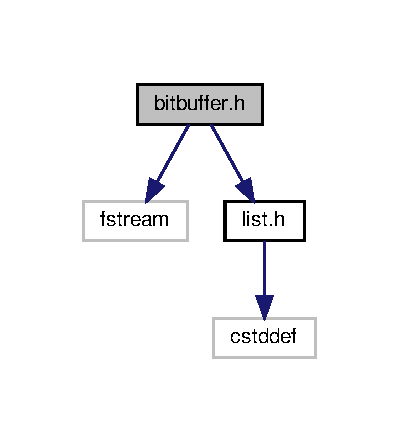
\includegraphics[width=192pt]{bitbuffer_8h__incl}
\end{center}
\end{figure}
This graph shows which files directly or indirectly include this file\+:
\nopagebreak
\begin{figure}[H]
\begin{center}
\leavevmode
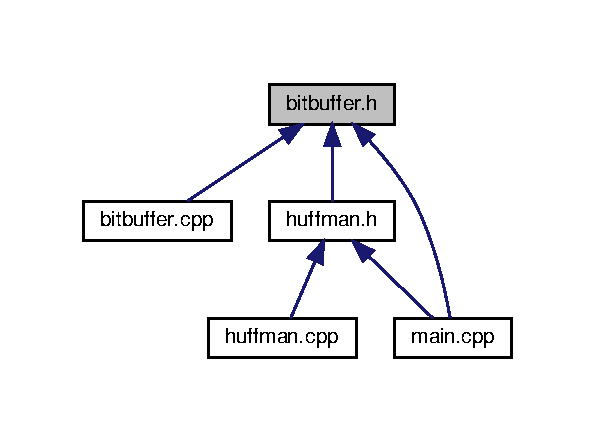
\includegraphics[width=286pt]{bitbuffer_8h__dep__incl}
\end{center}
\end{figure}
\subsection*{Classes}
\begin{DoxyCompactItemize}
\item 
class \textbf{ Bit\+Buffer}
\end{DoxyCompactItemize}

\hypertarget{gtest__lite_8h}{}\section{/home/ronaikovacs/\+Prog/\+C++/\+Prog2/hf/huffman\+\_\+1.2/gtest\+\_\+lite.h File Reference}
\label{gtest__lite_8h}\index{/home/ronaikovacs/\+Prog/\+C++/\+Prog2/hf/huffman\+\_\+1.\+2/gtest\+\_\+lite.\+h@{/home/ronaikovacs/\+Prog/\+C++/\+Prog2/hf/huffman\+\_\+1.\+2/gtest\+\_\+lite.\+h}}
{\ttfamily \#include $<$iostream$>$}\newline
{\ttfamily \#include $<$cassert$>$}\newline
{\ttfamily \#include $<$cmath$>$}\newline
{\ttfamily \#include $<$cstring$>$}\newline
{\ttfamily \#include $<$limits$>$}\newline
{\ttfamily \#include $<$string$>$}\newline
{\ttfamily \#include $<$fstream$>$}\newline
{\ttfamily \#include \char`\"{}memtrace.\+h\char`\"{}}\newline
\subsection*{Classes}
\begin{DoxyCompactItemize}
\item 
struct \hyperlink{struct___is___types}{\+\_\+\+Is\+\_\+\+Types$<$ F, T $>$}
\begin{DoxyCompactList}\small\item\em Segédsablon típuskonverzió futás közbeni ellenőrzésere. \end{DoxyCompactList}\item 
struct \hyperlink{structgtest__lite_1_1_test}{gtest\+\_\+lite\+::\+Test}
\end{DoxyCompactItemize}
\subsection*{Namespaces}
\begin{DoxyCompactItemize}
\item 
 \hyperlink{namespacegtest__lite}{gtest\+\_\+lite}
\begin{DoxyCompactList}\small\item\em \hyperlink{namespacegtest__lite}{gtest\+\_\+lite}\+: a keretrendszer függvényinek és objektumainak névtere \end{DoxyCompactList}\end{DoxyCompactItemize}
\subsection*{Macros}
\begin{DoxyCompactItemize}
\item 
\#define \hyperlink{gtest__lite_8h_a379a7b57e74521cb2c8e99f0e2779a72}{T\+E\+ST}(C,  N)~\{ gtest\+\_\+lite\+::test.\+begin(\#C\char`\"{}/\char`\"{}\#N);
\item 
\mbox{\Hypertarget{gtest__lite_8h_a29fd18bed01c4d836c7ebfe73a125c3f}\label{gtest__lite_8h_a29fd18bed01c4d836c7ebfe73a125c3f}} 
\#define \hyperlink{gtest__lite_8h_a29fd18bed01c4d836c7ebfe73a125c3f}{E\+ND}~gtest\+\_\+lite\+::test.\+end(); \}
\begin{DoxyCompactList}\small\item\em Teszteset vége. \end{DoxyCompactList}\item 
\#define \hyperlink{gtest__lite_8h_acc9065c889d0797062317b30fd8767d4}{E\+N\+DM}~gtest\+\_\+lite\+::test.\+end(true); \}
\item 
\#define \hyperlink{gtest__lite_8h_ad2e2f10cb2a494ff7ae23938dfdfc41a}{E\+N\+D\+Msg}(t)~gtest\+\_\+lite\+::test.\+end(true) $<$$<$ t $<$$<$ std\+::endl; \}
\item 
\mbox{\Hypertarget{gtest__lite_8h_a75adcdf89f69b0b615e395daafc315af}\label{gtest__lite_8h_a75adcdf89f69b0b615e395daafc315af}} 
\#define \hyperlink{gtest__lite_8h_a75adcdf89f69b0b615e395daafc315af}{S\+U\+C\+C\+E\+ED}()~gtest\+\_\+lite\+::test.\+expect(true, \+\_\+\+\_\+\+F\+I\+L\+E\+\_\+\+\_\+, \+\_\+\+\_\+\+L\+I\+N\+E\+\_\+\+\_\+, \char`\"{}S\+U\+C\+C\+E\+ED()\char`\"{}, true)
\begin{DoxyCompactList}\small\item\em Sikeres teszt makrója. \end{DoxyCompactList}\item 
\mbox{\Hypertarget{gtest__lite_8h_a3e26a8d27caa386ed0ea7ce9d5b7c4ed}\label{gtest__lite_8h_a3e26a8d27caa386ed0ea7ce9d5b7c4ed}} 
\#define \hyperlink{gtest__lite_8h_a3e26a8d27caa386ed0ea7ce9d5b7c4ed}{F\+A\+IL}()~gtest\+\_\+lite\+::test.\+expect(false, \+\_\+\+\_\+\+F\+I\+L\+E\+\_\+\+\_\+, \+\_\+\+\_\+\+L\+I\+N\+E\+\_\+\+\_\+, \char`\"{}F\+A\+IL()\char`\"{}, true)
\begin{DoxyCompactList}\small\item\em Sikertelen teszt makrója. \end{DoxyCompactList}\item 
\mbox{\Hypertarget{gtest__lite_8h_aff8385840165a184edc29446aa51936f}\label{gtest__lite_8h_aff8385840165a184edc29446aa51936f}} 
\#define \hyperlink{gtest__lite_8h_aff8385840165a184edc29446aa51936f}{E\+X\+P\+E\+C\+T\+\_\+\+EQ}(expected,  actual)~\hyperlink{namespacegtest__lite_ab358c162e1cedfc39abf5959417ffc1e}{gtest\+\_\+lite\+::\+E\+X\+P\+E\+C\+T\+\_\+}(expected, actual, \hyperlink{namespacegtest__lite_aa7762f23094d59c699ec402e1a37640c}{gtest\+\_\+lite\+::eq}, \+\_\+\+\_\+\+F\+I\+L\+E\+\_\+\+\_\+, \+\_\+\+\_\+\+L\+I\+N\+E\+\_\+\+\_\+, \char`\"{}E\+X\+P\+E\+C\+T\+\_\+\+EQ(\char`\"{} \#expected \char`\"{}, \char`\"{} \#actual \char`\"{})\char`\"{} )
\begin{DoxyCompactList}\small\item\em Azonosságot elváró makró \end{DoxyCompactList}\item 
\mbox{\Hypertarget{gtest__lite_8h_adb8a724f2c5c63ead11073c21fd51198}\label{gtest__lite_8h_adb8a724f2c5c63ead11073c21fd51198}} 
\#define \hyperlink{gtest__lite_8h_adb8a724f2c5c63ead11073c21fd51198}{E\+X\+P\+E\+C\+T\+\_\+\+NE}(expected,  actual)~\hyperlink{namespacegtest__lite_ab358c162e1cedfc39abf5959417ffc1e}{gtest\+\_\+lite\+::\+E\+X\+P\+E\+C\+T\+\_\+}(expected, actual, gtest\+\_\+lite\+::ne, \+\_\+\+\_\+\+F\+I\+L\+E\+\_\+\+\_\+, \+\_\+\+\_\+\+L\+I\+N\+E\+\_\+\+\_\+, \char`\"{}E\+X\+P\+E\+C\+T\+\_\+\+NE(\char`\"{} \#expected \char`\"{}, \char`\"{} \#actual \char`\"{})\char`\"{}, \char`\"{}etalon\char`\"{} )
\begin{DoxyCompactList}\small\item\em Eltérést elváró makró \end{DoxyCompactList}\item 
\mbox{\Hypertarget{gtest__lite_8h_ac680be4a2404c20cae831740779d11cd}\label{gtest__lite_8h_ac680be4a2404c20cae831740779d11cd}} 
\#define \hyperlink{gtest__lite_8h_ac680be4a2404c20cae831740779d11cd}{E\+X\+P\+E\+C\+T\+\_\+\+LE}(expected,  actual)~\hyperlink{namespacegtest__lite_ab358c162e1cedfc39abf5959417ffc1e}{gtest\+\_\+lite\+::\+E\+X\+P\+E\+C\+T\+\_\+}(expected, actual, gtest\+\_\+lite\+::le, \+\_\+\+\_\+\+F\+I\+L\+E\+\_\+\+\_\+, \+\_\+\+\_\+\+L\+I\+N\+E\+\_\+\+\_\+, \char`\"{}E\+X\+P\+E\+C\+T\+\_\+\+LE(\char`\"{} \#expected \char`\"{}, \char`\"{} \#actual \char`\"{})\char`\"{}, \char`\"{}etalon\char`\"{} )
\begin{DoxyCompactList}\small\item\em Kisebb, vagy egyenlő relációt elváró makró \end{DoxyCompactList}\item 
\mbox{\Hypertarget{gtest__lite_8h_a46603095284e7bcd2f114cfdc7c79b4f}\label{gtest__lite_8h_a46603095284e7bcd2f114cfdc7c79b4f}} 
\#define \hyperlink{gtest__lite_8h_a46603095284e7bcd2f114cfdc7c79b4f}{E\+X\+P\+E\+C\+T\+\_\+\+LT}(expected,  actual)~\hyperlink{namespacegtest__lite_ab358c162e1cedfc39abf5959417ffc1e}{gtest\+\_\+lite\+::\+E\+X\+P\+E\+C\+T\+\_\+}(expected, actual, gtest\+\_\+lite\+::lt, \+\_\+\+\_\+\+F\+I\+L\+E\+\_\+\+\_\+, \+\_\+\+\_\+\+L\+I\+N\+E\+\_\+\+\_\+, \char`\"{}E\+X\+P\+E\+C\+T\+\_\+\+LT(\char`\"{} \#expected \char`\"{}, \char`\"{} \#actual \char`\"{})\char`\"{}, \char`\"{}etalon\char`\"{} )
\begin{DoxyCompactList}\small\item\em Kisebb, mint relációt elváró makró \end{DoxyCompactList}\item 
\mbox{\Hypertarget{gtest__lite_8h_aad891c6b36689d35ee54de65351ab224}\label{gtest__lite_8h_aad891c6b36689d35ee54de65351ab224}} 
\#define \hyperlink{gtest__lite_8h_aad891c6b36689d35ee54de65351ab224}{E\+X\+P\+E\+C\+T\+\_\+\+GE}(expected,  actual)~\hyperlink{namespacegtest__lite_ab358c162e1cedfc39abf5959417ffc1e}{gtest\+\_\+lite\+::\+E\+X\+P\+E\+C\+T\+\_\+}(expected, actual, gtest\+\_\+lite\+::ge, \+\_\+\+\_\+\+F\+I\+L\+E\+\_\+\+\_\+, \+\_\+\+\_\+\+L\+I\+N\+E\+\_\+\+\_\+, \char`\"{}E\+X\+P\+E\+C\+T\+\_\+\+GE(\char`\"{} \#expected \char`\"{}, \char`\"{} \#actual \char`\"{})\char`\"{}, \char`\"{}etalon\char`\"{} )
\begin{DoxyCompactList}\small\item\em Nagyobb, vagy egyenlő relációt elváró makró \end{DoxyCompactList}\item 
\mbox{\Hypertarget{gtest__lite_8h_ac2262f96c4664cf3e170d2edaaba6c44}\label{gtest__lite_8h_ac2262f96c4664cf3e170d2edaaba6c44}} 
\#define \hyperlink{gtest__lite_8h_ac2262f96c4664cf3e170d2edaaba6c44}{E\+X\+P\+E\+C\+T\+\_\+\+GT}(expected,  actual)~\hyperlink{namespacegtest__lite_ab358c162e1cedfc39abf5959417ffc1e}{gtest\+\_\+lite\+::\+E\+X\+P\+E\+C\+T\+\_\+}(expected, actual, gtest\+\_\+lite\+::gt, \+\_\+\+\_\+\+F\+I\+L\+E\+\_\+\+\_\+, \+\_\+\+\_\+\+L\+I\+N\+E\+\_\+\+\_\+, \char`\"{}E\+X\+P\+E\+C\+T\+\_\+\+GT(\char`\"{} \#expected \char`\"{}, \char`\"{} \#actual \char`\"{})\char`\"{}, \char`\"{}etalon\char`\"{} )
\begin{DoxyCompactList}\small\item\em Nagyobb, mint relációt elváró makró \end{DoxyCompactList}\item 
\mbox{\Hypertarget{gtest__lite_8h_ab400890edc9f419e40c28a224e8ed79f}\label{gtest__lite_8h_ab400890edc9f419e40c28a224e8ed79f}} 
\#define \hyperlink{gtest__lite_8h_ab400890edc9f419e40c28a224e8ed79f}{E\+X\+P\+E\+C\+T\+\_\+\+T\+R\+UE}(actual)~\hyperlink{namespacegtest__lite_ab358c162e1cedfc39abf5959417ffc1e}{gtest\+\_\+lite\+::\+E\+X\+P\+E\+C\+T\+\_\+}(true, actual,  \hyperlink{namespacegtest__lite_aa7762f23094d59c699ec402e1a37640c}{gtest\+\_\+lite\+::eq}, \+\_\+\+\_\+\+F\+I\+L\+E\+\_\+\+\_\+, \+\_\+\+\_\+\+L\+I\+N\+E\+\_\+\+\_\+, \char`\"{}E\+X\+P\+E\+C\+T\+\_\+\+T\+R\+UE(\char`\"{} \#actual \char`\"{})\char`\"{} )
\begin{DoxyCompactList}\small\item\em Igaz értéket elváró makró \end{DoxyCompactList}\item 
\mbox{\Hypertarget{gtest__lite_8h_a58cae60fff88d713c4850b50d3e592a6}\label{gtest__lite_8h_a58cae60fff88d713c4850b50d3e592a6}} 
\#define \hyperlink{gtest__lite_8h_a58cae60fff88d713c4850b50d3e592a6}{E\+X\+P\+E\+C\+T\+\_\+\+F\+A\+L\+SE}(actual)~\hyperlink{namespacegtest__lite_ab358c162e1cedfc39abf5959417ffc1e}{gtest\+\_\+lite\+::\+E\+X\+P\+E\+C\+T\+\_\+}(false, actual, \hyperlink{namespacegtest__lite_aa7762f23094d59c699ec402e1a37640c}{gtest\+\_\+lite\+::eq}, \+\_\+\+\_\+\+F\+I\+L\+E\+\_\+\+\_\+, \+\_\+\+\_\+\+L\+I\+N\+E\+\_\+\+\_\+, \char`\"{}E\+X\+P\+E\+C\+T\+\_\+\+F\+A\+L\+SE(\char`\"{} \#actual \char`\"{})\char`\"{} )
\begin{DoxyCompactList}\small\item\em Hamis értéket elváró makró \end{DoxyCompactList}\item 
\mbox{\Hypertarget{gtest__lite_8h_a5ce7d58df8cb696aa05e77c2370de7a8}\label{gtest__lite_8h_a5ce7d58df8cb696aa05e77c2370de7a8}} 
\#define \hyperlink{gtest__lite_8h_a5ce7d58df8cb696aa05e77c2370de7a8}{E\+X\+P\+E\+C\+T\+\_\+\+F\+L\+O\+A\+T\+\_\+\+EQ}(expected,  actual)~\hyperlink{namespacegtest__lite_ab358c162e1cedfc39abf5959417ffc1e}{gtest\+\_\+lite\+::\+E\+X\+P\+E\+C\+T\+\_\+}(expected, actual, \hyperlink{namespacegtest__lite_affbf9748c4e4dec6db137f7c147fee61}{gtest\+\_\+lite\+::almost\+EQ}, \+\_\+\+\_\+\+F\+I\+L\+E\+\_\+\+\_\+, \+\_\+\+\_\+\+L\+I\+N\+E\+\_\+\+\_\+, \char`\"{}E\+X\+P\+E\+C\+T\+\_\+\+F\+L\+O\+A\+T\+\_\+\+EQ(\char`\"{} \#expected \char`\"{}, \char`\"{} \#actual \char`\"{})\char`\"{} )
\begin{DoxyCompactList}\small\item\em Valós számok azonosságát elváró makró \end{DoxyCompactList}\item 
\mbox{\Hypertarget{gtest__lite_8h_a6e6277442d96cd18300619c321614397}\label{gtest__lite_8h_a6e6277442d96cd18300619c321614397}} 
\#define \hyperlink{gtest__lite_8h_a6e6277442d96cd18300619c321614397}{E\+X\+P\+E\+C\+T\+\_\+\+D\+O\+U\+B\+L\+E\+\_\+\+EQ}(expected,  actual)~\hyperlink{namespacegtest__lite_ab358c162e1cedfc39abf5959417ffc1e}{gtest\+\_\+lite\+::\+E\+X\+P\+E\+C\+T\+\_\+}(expected, actual, \hyperlink{namespacegtest__lite_affbf9748c4e4dec6db137f7c147fee61}{gtest\+\_\+lite\+::almost\+EQ}, \+\_\+\+\_\+\+F\+I\+L\+E\+\_\+\+\_\+, \+\_\+\+\_\+\+L\+I\+N\+E\+\_\+\+\_\+, \char`\"{}E\+X\+P\+E\+C\+T\+\_\+\+D\+O\+U\+B\+L\+E\+\_\+\+EQ(\char`\"{} \#expected \char`\"{}, \char`\"{} \#actual \char`\"{})\char`\"{} )
\begin{DoxyCompactList}\small\item\em Valós számok azonosságát elváró makró \end{DoxyCompactList}\item 
\mbox{\Hypertarget{gtest__lite_8h_a5b4b193a92c39b99d7b9404c49feef0b}\label{gtest__lite_8h_a5b4b193a92c39b99d7b9404c49feef0b}} 
\#define \hyperlink{gtest__lite_8h_a5b4b193a92c39b99d7b9404c49feef0b}{E\+X\+P\+E\+C\+T\+\_\+\+S\+T\+R\+EQ}(expected,  actual)~\hyperlink{namespacegtest__lite_aea477921e4c26d2a2806bc3011066270}{gtest\+\_\+lite\+::\+E\+X\+P\+E\+C\+T\+S\+TR}(expected, actual, gtest\+\_\+lite\+::eqstr, \+\_\+\+\_\+\+F\+I\+L\+E\+\_\+\+\_\+, \+\_\+\+\_\+\+L\+I\+N\+E\+\_\+\+\_\+, \char`\"{}E\+X\+P\+E\+C\+T\+\_\+\+S\+T\+R\+EQ(\char`\"{} \#expected \char`\"{}, \char`\"{} \#actual \char`\"{})\char`\"{} )
\begin{DoxyCompactList}\small\item\em C stringek (const char $\ast$) azonosságát tesztelő makró \end{DoxyCompactList}\item 
\mbox{\Hypertarget{gtest__lite_8h_aa511aad7b6a6a8e8d0279f16d925b094}\label{gtest__lite_8h_aa511aad7b6a6a8e8d0279f16d925b094}} 
\#define \hyperlink{gtest__lite_8h_aa511aad7b6a6a8e8d0279f16d925b094}{E\+X\+P\+E\+C\+T\+\_\+\+S\+T\+R\+NE}(expected,  actual)~\hyperlink{namespacegtest__lite_aea477921e4c26d2a2806bc3011066270}{gtest\+\_\+lite\+::\+E\+X\+P\+E\+C\+T\+S\+TR}(expected, actual, gtest\+\_\+lite\+::nestr, \+\_\+\+\_\+\+F\+I\+L\+E\+\_\+\+\_\+, \+\_\+\+\_\+\+L\+I\+N\+E\+\_\+\+\_\+, \char`\"{}E\+X\+P\+E\+C\+T\+\_\+\+S\+T\+R\+NE(\char`\"{} \#expected \char`\"{}, \char`\"{} \#actual \char`\"{})\char`\"{}, \char`\"{}etalon\char`\"{} )
\begin{DoxyCompactList}\small\item\em C stringek (const char $\ast$) eltéréset tesztelő makró \end{DoxyCompactList}\item 
\#define \hyperlink{gtest__lite_8h_a4b4fe697f312ef7d2618905a9bc12f04}{E\+X\+P\+E\+C\+T\+\_\+\+T\+H\+R\+OW}(statement,  exception\+\_\+type)
\begin{DoxyCompactList}\small\item\em Kivételt várunk. \end{DoxyCompactList}\item 
\#define \hyperlink{gtest__lite_8h_a9be43f44d148e8a8d6a89c864bf4e461}{E\+X\+P\+E\+C\+T\+\_\+\+A\+N\+Y\+\_\+\+T\+H\+R\+OW}(statement)
\begin{DoxyCompactList}\small\item\em Kivételt várunk. \end{DoxyCompactList}\item 
\#define \hyperlink{gtest__lite_8h_a2743a1438137ad857aa3f9fec3ff67ec}{E\+X\+P\+E\+C\+T\+\_\+\+N\+O\+\_\+\+T\+H\+R\+OW}(statement)
\begin{DoxyCompactList}\small\item\em Nem várunk kivételt. \end{DoxyCompactList}\item 
\#define \hyperlink{gtest__lite_8h_a5129ea3a961fbd7fe71e6621452047bf}{E\+X\+P\+E\+C\+T\+\_\+\+T\+H\+R\+O\+W\+\_\+\+T\+H\+R\+OW}(statement,  exception\+\_\+type)
\begin{DoxyCompactList}\small\item\em Kivételt várunk és továbbdobjuk -- ilyen nincs a gtest-\/ben. \end{DoxyCompactList}\item 
\#define \hyperlink{gtest__lite_8h_a34bf9a881eb6b2800b0e6cb0abdbd319}{C\+R\+E\+A\+T\+E\+\_\+\+Has\+\_\+}(X)
\item 
\#define \hyperlink{gtest__lite_8h_a59f6c1f1654aa9d5adf5c143efd1a454}{E\+X\+P\+E\+C\+T\+T\+H\+R\+OW}(statement,  exp,  act)
\begin{DoxyCompactList}\small\item\em E\+X\+P\+E\+C\+T\+T\+H\+R\+OW\+: kivételkezelés. \end{DoxyCompactList}\item 
\mbox{\Hypertarget{gtest__lite_8h_a428e5e5ea2b7f67a0b68fbf57ea0faa7}\label{gtest__lite_8h_a428e5e5ea2b7f67a0b68fbf57ea0faa7}} 
\#define {\bfseries G\+T\+I\+N\+IT}(IS)
\item 
\mbox{\Hypertarget{gtest__lite_8h_a20ba54bca307f985eb448f71e6896dd5}\label{gtest__lite_8h_a20ba54bca307f985eb448f71e6896dd5}} 
\#define {\bfseries G\+T\+E\+ND}(os)
\end{DoxyCompactItemize}
\subsection*{Functions}
\begin{DoxyCompactItemize}
\item 
\mbox{\Hypertarget{namespacegtest__lite_ab358c162e1cedfc39abf5959417ffc1e}\label{namespacegtest__lite_ab358c162e1cedfc39abf5959417ffc1e}} 
{\footnotesize template$<$typename T $>$ }\\std\+::ostream \& \hyperlink{namespacegtest__lite_ab358c162e1cedfc39abf5959417ffc1e}{gtest\+\_\+lite\+::\+E\+X\+P\+E\+C\+T\+\_\+} (T exp, T act, bool($\ast$pred)(T, T), const char $\ast$file, int line, const char $\ast$expr, const char $\ast$lhs=\char`\"{}elvart\char`\"{}, const char $\ast$rhs=\char`\"{}aktual\char`\"{})
\begin{DoxyCompactList}\small\item\em általános sablon a várt értékhez. \end{DoxyCompactList}\item 
\mbox{\Hypertarget{namespacegtest__lite_a8b21cff4e93dcacdd1b4fdb8b6b9c740}\label{namespacegtest__lite_a8b21cff4e93dcacdd1b4fdb8b6b9c740}} 
{\footnotesize template$<$typename T $>$ }\\std\+::ostream \& \hyperlink{namespacegtest__lite_a8b21cff4e93dcacdd1b4fdb8b6b9c740}{gtest\+\_\+lite\+::\+E\+X\+P\+E\+C\+T\+\_\+} (T $\ast$exp, T $\ast$act, bool($\ast$pred)(T $\ast$, T $\ast$), const char $\ast$file, int line, const char $\ast$expr, const char $\ast$lhs=\char`\"{}elvart\char`\"{}, const char $\ast$rhs=\char`\"{}aktual\char`\"{})
\begin{DoxyCompactList}\small\item\em pointerre specializált sablon a várt értékhez. \end{DoxyCompactList}\item 
std\+::ostream \& \hyperlink{namespacegtest__lite_aea477921e4c26d2a2806bc3011066270}{gtest\+\_\+lite\+::\+E\+X\+P\+E\+C\+T\+S\+TR} (const char $\ast$exp, const char $\ast$act, bool($\ast$pred)(const char $\ast$, const char $\ast$), const char $\ast$file, int line, const char $\ast$expr, const char $\ast$lhs=\char`\"{}elvart\char`\"{}, const char $\ast$rhs=\char`\"{}aktual\char`\"{})
\item 
{\footnotesize template$<$typename T $>$ }\\bool \hyperlink{namespacegtest__lite_aa7762f23094d59c699ec402e1a37640c}{gtest\+\_\+lite\+::eq} (T a, T b)
\item 
\mbox{\Hypertarget{namespacegtest__lite_a34055f353dabbe4ed9063f1d36af6022}\label{namespacegtest__lite_a34055f353dabbe4ed9063f1d36af6022}} 
bool {\bfseries gtest\+\_\+lite\+::eqstr} (const char $\ast$a, const char $\ast$b)
\item 
\mbox{\Hypertarget{namespacegtest__lite_a9a1485affebbed604f7cac69f70072dc}\label{namespacegtest__lite_a9a1485affebbed604f7cac69f70072dc}} 
{\footnotesize template$<$typename T $>$ }\\bool {\bfseries gtest\+\_\+lite\+::ne} (T a, T b)
\item 
\mbox{\Hypertarget{namespacegtest__lite_a0a34b1bb0d55bc0c6a3e878ec2bcd49f}\label{namespacegtest__lite_a0a34b1bb0d55bc0c6a3e878ec2bcd49f}} 
bool {\bfseries gtest\+\_\+lite\+::nestr} (const char $\ast$a, const char $\ast$b)
\item 
\mbox{\Hypertarget{namespacegtest__lite_a92068d494867b61abeef5942eefac3a3}\label{namespacegtest__lite_a92068d494867b61abeef5942eefac3a3}} 
{\footnotesize template$<$typename T $>$ }\\bool {\bfseries gtest\+\_\+lite\+::le} (T a, T b)
\item 
\mbox{\Hypertarget{namespacegtest__lite_acfefb55c5d3713c79b659bbd18d9423c}\label{namespacegtest__lite_acfefb55c5d3713c79b659bbd18d9423c}} 
{\footnotesize template$<$typename T $>$ }\\bool {\bfseries gtest\+\_\+lite\+::lt} (T a, T b)
\item 
\mbox{\Hypertarget{namespacegtest__lite_ae8c2517b99b688c6136d8c7c18551da5}\label{namespacegtest__lite_ae8c2517b99b688c6136d8c7c18551da5}} 
{\footnotesize template$<$typename T $>$ }\\bool {\bfseries gtest\+\_\+lite\+::ge} (T a, T b)
\item 
\mbox{\Hypertarget{namespacegtest__lite_a2075d101da98f80f569b0737c5185718}\label{namespacegtest__lite_a2075d101da98f80f569b0737c5185718}} 
{\footnotesize template$<$typename T $>$ }\\bool {\bfseries gtest\+\_\+lite\+::gt} (T a, T b)
\item 
{\footnotesize template$<$typename T $>$ }\\bool \hyperlink{namespacegtest__lite_affbf9748c4e4dec6db137f7c147fee61}{gtest\+\_\+lite\+::almost\+EQ} (T a, T b)
\end{DoxyCompactItemize}


\subsection{Detailed Description}
(v2)

Google gtest keretrendszerhez hasonló rendszer. Sz.\+I. 2015., 2016., 2017. (\+\_\+\+Has\+\_\+X) Sz.\+I. 2018 (template), E\+N\+DM, E\+N\+D\+Msg

A tesztelés legalapvetőbb funkcióit támogató függvények és makrók. Nem szálbiztos megvalósítás.

Egyetlen fájlban kell megvalósítani minden tesztesetet! Csak ebből include-\/olható a \hyperlink{gtest__lite_8h}{gtest\+\_\+lite.\+h} Ezen korlátozás kiküszöböléséhez sigletonnal kellene rednesen megvalósítani. a test osztályt!

Szabadon felhasználható, bővíthető.

Használati példa\+: Teszteljük az f(x)=2$\ast$x függvényt\+: int f(int x) \{ return 2$\ast$x; \}

int main() \{ \hyperlink{gtest__lite_8h_a379a7b57e74521cb2c8e99f0e2779a72}{T\+E\+S\+T(\+Tesz\+Eset\+Neve, Teszt\+Neve)} \hyperlink{gtest__lite_8h_aff8385840165a184edc29446aa51936f}{E\+X\+P\+E\+C\+T\+\_\+\+E\+Q(0, f(0))}; \hyperlink{gtest__lite_8h_aff8385840165a184edc29446aa51936f}{E\+X\+P\+E\+C\+T\+\_\+\+E\+Q(4, f(2))} $<$$<$ \char`\"{}\+A függvény hibás eredményt adott\char`\"{} $<$$<$ std\+::endl; ... E\+ND ...

A működés részleteinek megértése szorgalmi feladat. 

\subsection{Macro Definition Documentation}
\mbox{\Hypertarget{gtest__lite_8h_a34bf9a881eb6b2800b0e6cb0abdbd319}\label{gtest__lite_8h_a34bf9a881eb6b2800b0e6cb0abdbd319}} 
\index{gtest\+\_\+lite.\+h@{gtest\+\_\+lite.\+h}!C\+R\+E\+A\+T\+E\+\_\+\+Has\+\_\+@{C\+R\+E\+A\+T\+E\+\_\+\+Has\+\_\+}}
\index{C\+R\+E\+A\+T\+E\+\_\+\+Has\+\_\+@{C\+R\+E\+A\+T\+E\+\_\+\+Has\+\_\+}!gtest\+\_\+lite.\+h@{gtest\+\_\+lite.\+h}}
\subsubsection{\texorpdfstring{C\+R\+E\+A\+T\+E\+\_\+\+Has\+\_\+}{CREATE\_Has\_}}
{\footnotesize\ttfamily \#define C\+R\+E\+A\+T\+E\+\_\+\+Has\+\_\+(\begin{DoxyParamCaption}\item[{}]{X }\end{DoxyParamCaption})}

{\bfseries Value\+:}
\begin{DoxyCode}
\textcolor{keyword}{template}<\textcolor{keyword}{typename} T> \textcolor{keyword}{struct }\_Has\_##X \{  \(\backslash\)
    struct Fallback \{ \textcolor{keywordtype}{int} X; \};         \(\backslash\)
    struct Derived : T, Fallback \{\};    \(\backslash\)
    template<typename C, C> \textcolor{keyword}{struct }ChT; \(\backslash\)
    template<typename D> \textcolor{keyword}{static} char (&f(ChT<int Fallback::*, &D::X>*))[1]; \(\backslash\)
    template<typename D> \textcolor{keyword}{static} char (&f(...))[2]; \(\backslash\)
    static \textcolor{keywordtype}{bool} \textcolor{keyword}{const} member = \textcolor{keyword}{sizeof}(f<Derived>(0)) == 2; \(\backslash\)
\};
\end{DoxyCode}
Segédmakró egy adattag, vagy tagfüggvény létezésének tesztelésére futási időben Ötlet\+: \href{https://cpptalk.wordpress.com/2009/09/12/substitution-failure-is-not-an-error-2}{\tt https\+://cpptalk.\+wordpress.\+com/2009/09/12/substitution-\/failure-\/is-\/not-\/an-\/error-\/2} Használat\+: \hyperlink{gtest__lite_8h_a34bf9a881eb6b2800b0e6cb0abdbd319}{C\+R\+E\+A\+T\+E\+\_\+\+Has\+\_\+(size)} ... if (Has\+\_\+size$<$std\+::string$>$\+::member)... \mbox{\Hypertarget{gtest__lite_8h_acc9065c889d0797062317b30fd8767d4}\label{gtest__lite_8h_acc9065c889d0797062317b30fd8767d4}} 
\index{gtest\+\_\+lite.\+h@{gtest\+\_\+lite.\+h}!E\+N\+DM@{E\+N\+DM}}
\index{E\+N\+DM@{E\+N\+DM}!gtest\+\_\+lite.\+h@{gtest\+\_\+lite.\+h}}
\subsubsection{\texorpdfstring{E\+N\+DM}{ENDM}}
{\footnotesize\ttfamily \#define E\+N\+DM~gtest\+\_\+lite\+::test.\+end(true); \}}

Teszteset vége allokált blokkok számának összehasonlításával Ez az ellenőrzés nem bomba biztos. \mbox{\Hypertarget{gtest__lite_8h_ad2e2f10cb2a494ff7ae23938dfdfc41a}\label{gtest__lite_8h_ad2e2f10cb2a494ff7ae23938dfdfc41a}} 
\index{gtest\+\_\+lite.\+h@{gtest\+\_\+lite.\+h}!E\+N\+D\+Msg@{E\+N\+D\+Msg}}
\index{E\+N\+D\+Msg@{E\+N\+D\+Msg}!gtest\+\_\+lite.\+h@{gtest\+\_\+lite.\+h}}
\subsubsection{\texorpdfstring{E\+N\+D\+Msg}{ENDMsg}}
{\footnotesize\ttfamily \#define E\+N\+D\+Msg(\begin{DoxyParamCaption}\item[{}]{t }\end{DoxyParamCaption})~gtest\+\_\+lite\+::test.\+end(true) $<$$<$ t $<$$<$ std\+::endl; \}}

Teszteset vége allokált blokkok számának összehasonlításával Ez az ellenőrzés nem bomba biztos. Ha hiba van kiírja az üzenetet. \mbox{\Hypertarget{gtest__lite_8h_a9be43f44d148e8a8d6a89c864bf4e461}\label{gtest__lite_8h_a9be43f44d148e8a8d6a89c864bf4e461}} 
\index{gtest\+\_\+lite.\+h@{gtest\+\_\+lite.\+h}!E\+X\+P\+E\+C\+T\+\_\+\+A\+N\+Y\+\_\+\+T\+H\+R\+OW@{E\+X\+P\+E\+C\+T\+\_\+\+A\+N\+Y\+\_\+\+T\+H\+R\+OW}}
\index{E\+X\+P\+E\+C\+T\+\_\+\+A\+N\+Y\+\_\+\+T\+H\+R\+OW@{E\+X\+P\+E\+C\+T\+\_\+\+A\+N\+Y\+\_\+\+T\+H\+R\+OW}!gtest\+\_\+lite.\+h@{gtest\+\_\+lite.\+h}}
\subsubsection{\texorpdfstring{E\+X\+P\+E\+C\+T\+\_\+\+A\+N\+Y\+\_\+\+T\+H\+R\+OW}{EXPECT\_ANY\_THROW}}
{\footnotesize\ttfamily \#define E\+X\+P\+E\+C\+T\+\_\+\+A\+N\+Y\+\_\+\+T\+H\+R\+OW(\begin{DoxyParamCaption}\item[{}]{statement }\end{DoxyParamCaption})}

{\bfseries Value\+:}
\begin{DoxyCode}
\textcolor{keywordflow}{try} \{ gtest\_lite::test.\hyperlink{structgtest__lite_1_1_test_a1145ceb335a60a808b7b4d5d1624b2a5}{tmp} = \textcolor{keyword}{false}; statement; \} \(\backslash\)
    catch (...) \{ gtest\_lite::test.\hyperlink{structgtest__lite_1_1_test_a1145ceb335a60a808b7b4d5d1624b2a5}{tmp} = \textcolor{keyword}{true}; \} \(\backslash\)
    EXPECTTHROW(statement, \textcolor{stringliteral}{"kivetelt dob."}, \textcolor{stringliteral}{"nem dobott kivetelt."})
\end{DoxyCode}


Kivételt várunk. 

\mbox{\Hypertarget{gtest__lite_8h_a2743a1438137ad857aa3f9fec3ff67ec}\label{gtest__lite_8h_a2743a1438137ad857aa3f9fec3ff67ec}} 
\index{gtest\+\_\+lite.\+h@{gtest\+\_\+lite.\+h}!E\+X\+P\+E\+C\+T\+\_\+\+N\+O\+\_\+\+T\+H\+R\+OW@{E\+X\+P\+E\+C\+T\+\_\+\+N\+O\+\_\+\+T\+H\+R\+OW}}
\index{E\+X\+P\+E\+C\+T\+\_\+\+N\+O\+\_\+\+T\+H\+R\+OW@{E\+X\+P\+E\+C\+T\+\_\+\+N\+O\+\_\+\+T\+H\+R\+OW}!gtest\+\_\+lite.\+h@{gtest\+\_\+lite.\+h}}
\subsubsection{\texorpdfstring{E\+X\+P\+E\+C\+T\+\_\+\+N\+O\+\_\+\+T\+H\+R\+OW}{EXPECT\_NO\_THROW}}
{\footnotesize\ttfamily \#define E\+X\+P\+E\+C\+T\+\_\+\+N\+O\+\_\+\+T\+H\+R\+OW(\begin{DoxyParamCaption}\item[{}]{statement }\end{DoxyParamCaption})}

{\bfseries Value\+:}
\begin{DoxyCode}
\textcolor{keywordflow}{try} \{ gtest\_lite::test.\hyperlink{structgtest__lite_1_1_test_a1145ceb335a60a808b7b4d5d1624b2a5}{tmp} = \textcolor{keyword}{true}; statement; \} \(\backslash\)
    catch (...) \{ gtest\_lite::test.\hyperlink{structgtest__lite_1_1_test_a1145ceb335a60a808b7b4d5d1624b2a5}{tmp} = \textcolor{keyword}{false}; \}\(\backslash\)
    EXPECTTHROW(statement, \textcolor{stringliteral}{"nem dob kivetelt."}, \textcolor{stringliteral}{"kivetelt dobott."})
\end{DoxyCode}


Nem várunk kivételt. 

\mbox{\Hypertarget{gtest__lite_8h_a4b4fe697f312ef7d2618905a9bc12f04}\label{gtest__lite_8h_a4b4fe697f312ef7d2618905a9bc12f04}} 
\index{gtest\+\_\+lite.\+h@{gtest\+\_\+lite.\+h}!E\+X\+P\+E\+C\+T\+\_\+\+T\+H\+R\+OW@{E\+X\+P\+E\+C\+T\+\_\+\+T\+H\+R\+OW}}
\index{E\+X\+P\+E\+C\+T\+\_\+\+T\+H\+R\+OW@{E\+X\+P\+E\+C\+T\+\_\+\+T\+H\+R\+OW}!gtest\+\_\+lite.\+h@{gtest\+\_\+lite.\+h}}
\subsubsection{\texorpdfstring{E\+X\+P\+E\+C\+T\+\_\+\+T\+H\+R\+OW}{EXPECT\_THROW}}
{\footnotesize\ttfamily \#define E\+X\+P\+E\+C\+T\+\_\+\+T\+H\+R\+OW(\begin{DoxyParamCaption}\item[{}]{statement,  }\item[{}]{exception\+\_\+type }\end{DoxyParamCaption})}

{\bfseries Value\+:}
\begin{DoxyCode}
\textcolor{keywordflow}{try} \{ gtest\_lite::test.\hyperlink{structgtest__lite_1_1_test_a1145ceb335a60a808b7b4d5d1624b2a5}{tmp} = \textcolor{keyword}{false}; statement; \} \(\backslash\)
    catch (exception\_type) \{ gtest\_lite::test.\hyperlink{structgtest__lite_1_1_test_a1145ceb335a60a808b7b4d5d1624b2a5}{tmp} = \textcolor{keyword}{true}; \} \(\backslash\)
    catch (...) \{ \} \(\backslash\)
    EXPECTTHROW(statement, \textcolor{stringliteral}{"kivetelt dob."}, \textcolor{stringliteral}{"nem dobott '"}#exception\_type\textcolor{stringliteral}{"' kivetelt."})
\end{DoxyCode}


Kivételt várunk. 

\mbox{\Hypertarget{gtest__lite_8h_a5129ea3a961fbd7fe71e6621452047bf}\label{gtest__lite_8h_a5129ea3a961fbd7fe71e6621452047bf}} 
\index{gtest\+\_\+lite.\+h@{gtest\+\_\+lite.\+h}!E\+X\+P\+E\+C\+T\+\_\+\+T\+H\+R\+O\+W\+\_\+\+T\+H\+R\+OW@{E\+X\+P\+E\+C\+T\+\_\+\+T\+H\+R\+O\+W\+\_\+\+T\+H\+R\+OW}}
\index{E\+X\+P\+E\+C\+T\+\_\+\+T\+H\+R\+O\+W\+\_\+\+T\+H\+R\+OW@{E\+X\+P\+E\+C\+T\+\_\+\+T\+H\+R\+O\+W\+\_\+\+T\+H\+R\+OW}!gtest\+\_\+lite.\+h@{gtest\+\_\+lite.\+h}}
\subsubsection{\texorpdfstring{E\+X\+P\+E\+C\+T\+\_\+\+T\+H\+R\+O\+W\+\_\+\+T\+H\+R\+OW}{EXPECT\_THROW\_THROW}}
{\footnotesize\ttfamily \#define E\+X\+P\+E\+C\+T\+\_\+\+T\+H\+R\+O\+W\+\_\+\+T\+H\+R\+OW(\begin{DoxyParamCaption}\item[{}]{statement,  }\item[{}]{exception\+\_\+type }\end{DoxyParamCaption})}

{\bfseries Value\+:}
\begin{DoxyCode}
\textcolor{keywordflow}{try} \{ gtest\_lite::test.\hyperlink{structgtest__lite_1_1_test_a1145ceb335a60a808b7b4d5d1624b2a5}{tmp} = \textcolor{keyword}{false}; statement; \} \(\backslash\)
    catch (exception\_type) \{ gtest\_lite::test.\hyperlink{structgtest__lite_1_1_test_a1145ceb335a60a808b7b4d5d1624b2a5}{tmp} = \textcolor{keyword}{true}; \textcolor{keywordflow}{throw}; \} \(\backslash\)
    EXPECTTHROW(statement, \textcolor{stringliteral}{"kivetelt dob."}, \textcolor{stringliteral}{"nem dobott '"}#exception\_type\textcolor{stringliteral}{"' kivetelt."})
\end{DoxyCode}


Kivételt várunk és továbbdobjuk -- ilyen nincs a gtest-\/ben. 

\mbox{\Hypertarget{gtest__lite_8h_a59f6c1f1654aa9d5adf5c143efd1a454}\label{gtest__lite_8h_a59f6c1f1654aa9d5adf5c143efd1a454}} 
\index{gtest\+\_\+lite.\+h@{gtest\+\_\+lite.\+h}!E\+X\+P\+E\+C\+T\+T\+H\+R\+OW@{E\+X\+P\+E\+C\+T\+T\+H\+R\+OW}}
\index{E\+X\+P\+E\+C\+T\+T\+H\+R\+OW@{E\+X\+P\+E\+C\+T\+T\+H\+R\+OW}!gtest\+\_\+lite.\+h@{gtest\+\_\+lite.\+h}}
\subsubsection{\texorpdfstring{E\+X\+P\+E\+C\+T\+T\+H\+R\+OW}{EXPECTTHROW}}
{\footnotesize\ttfamily \#define E\+X\+P\+E\+C\+T\+T\+H\+R\+OW(\begin{DoxyParamCaption}\item[{}]{statement,  }\item[{}]{exp,  }\item[{}]{act }\end{DoxyParamCaption})}

{\bfseries Value\+:}
\begin{DoxyCode}
gtest\_lite::test.\hyperlink{structgtest__lite_1_1_test_a0bca03315e5963f7fdfffd92d2daed6a}{expect}(gtest\_lite::test.tmp, \_\_FILE\_\_, \_\_LINE\_\_, #statement) \(\backslash\)
    << \textcolor{stringliteral}{"** Az utasitas "} << (act) \(\backslash\)
    << \textcolor{stringliteral}{"\(\backslash\)n** Azt vartuk, hogy "} << (exp) << std::endl
\end{DoxyCode}


E\+X\+P\+E\+C\+T\+T\+H\+R\+OW\+: kivételkezelés. 



 Belső megvalósításhoz tartozó makrók, és osztályok. \subsubsection*{Nem célszerű közvetlenül használni, vagy módosítani }\mbox{\Hypertarget{gtest__lite_8h_a379a7b57e74521cb2c8e99f0e2779a72}\label{gtest__lite_8h_a379a7b57e74521cb2c8e99f0e2779a72}} 
\index{gtest\+\_\+lite.\+h@{gtest\+\_\+lite.\+h}!T\+E\+ST@{T\+E\+ST}}
\index{T\+E\+ST@{T\+E\+ST}!gtest\+\_\+lite.\+h@{gtest\+\_\+lite.\+h}}
\subsubsection{\texorpdfstring{T\+E\+ST}{TEST}}
{\footnotesize\ttfamily \#define T\+E\+ST(\begin{DoxyParamCaption}\item[{}]{C,  }\item[{}]{N }\end{DoxyParamCaption})~\{ gtest\+\_\+lite\+::test.\+begin(\#C\char`\"{}/\char`\"{}\#N);}

Teszt kezdete. A makró paraméterezése hasonlít a gtest paraméterezéséhez. Így az itt elkészített testek könnyen átemelhetők a gtest keretrendszerbe. 
\begin{DoxyParams}{Parameters}
{\em C} & -\/ teszteset neve (csak a gtest kompatibilitás miatt van külön neve az eseteknek) \\
\hline
{\em N} & -\/ teszt neve \\
\hline
\end{DoxyParams}

\hypertarget{huffman_8cpp}{}\section{huffman.\+cpp File Reference}
\label{huffman_8cpp}\index{huffman.\+cpp@{huffman.\+cpp}}
{\ttfamily \#include \char`\"{}memtrace.\+h\char`\"{}}\newline
{\ttfamily \#include \char`\"{}huffman.\+h\char`\"{}}\newline
{\ttfamily \#include \char`\"{}node.\+h\char`\"{}}\newline

\hypertarget{huffman_8h}{}\section{huffman.\+h File Reference}
\label{huffman_8h}\index{huffman.\+h@{huffman.\+h}}
{\ttfamily \#include $<$iostream$>$}\newline
{\ttfamily \#include $<$fstream$>$}\newline
{\ttfamily \#include $<$cstdlib$>$}\newline
{\ttfamily \#include $<$cstring$>$}\newline
{\ttfamily \#include $<$utility$>$}\newline
{\ttfamily \#include \char`\"{}list.\+h\char`\"{}}\newline
{\ttfamily \#include \char`\"{}node.\+h\char`\"{}}\newline
{\ttfamily \#include \char`\"{}bitbuffer.\+h\char`\"{}}\newline
\subsection*{Classes}
\begin{DoxyCompactItemize}
\item 
class \hyperlink{class_huffman}{Huffman}
\end{DoxyCompactItemize}

\section{letter.\+h File Reference}
\label{letter_8h}\index{letter.\+h@{letter.\+h}}
This graph shows which files directly or indirectly include this file\+:
\nopagebreak
\begin{figure}[H]
\begin{center}
\leavevmode
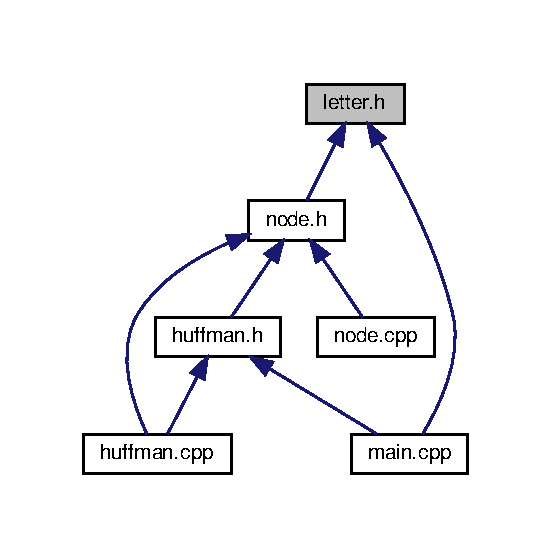
\includegraphics[width=265pt]{letter_8h__dep__incl}
\end{center}
\end{figure}
\subsection*{Classes}
\begin{DoxyCompactItemize}
\item 
class \textbf{ Letter}
\end{DoxyCompactItemize}

\section{list.\+cpp File Reference}
\label{list_8cpp}\index{list.\+cpp@{list.\+cpp}}
{\ttfamily \#include \char`\"{}list.\+h\char`\"{}}\newline
Include dependency graph for list.\+cpp\+:
\nopagebreak
\begin{figure}[H]
\begin{center}
\leavevmode
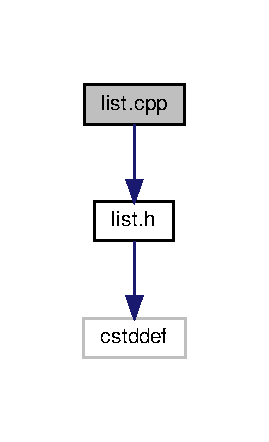
\includegraphics[width=129pt]{list_8cpp__incl}
\end{center}
\end{figure}

\hypertarget{list_8h}{}\section{list.\+h File Reference}
\label{list_8h}\index{list.\+h@{list.\+h}}
{\ttfamily \#include $<$cstddef$>$}\newline
\subsection*{Classes}
\begin{DoxyCompactItemize}
\item 
class \hyperlink{class_list}{List$<$ T $>$}
\end{DoxyCompactItemize}

\hypertarget{main_8cpp}{}\section{main.\+cpp File Reference}
\label{main_8cpp}\index{main.\+cpp@{main.\+cpp}}
{\ttfamily \#include $<$iostream$>$}\newline
{\ttfamily \#include \char`\"{}gtest\+\_\+lite.\+h\char`\"{}}\newline
{\ttfamily \#include \char`\"{}memtrace.\+h\char`\"{}}\newline
{\ttfamily \#include \char`\"{}bitbuffer.\+h\char`\"{}}\newline
{\ttfamily \#include \char`\"{}letter.\+h\char`\"{}}\newline
{\ttfamily \#include \char`\"{}huffman.\+h\char`\"{}}\newline
\subsection*{Macros}
\begin{DoxyCompactItemize}
\item 
\#define \hyperlink{main_8cpp_a05a1e28ae45a774fa1a2b84c46a5928e}{H\+U\+F\+F\+M\+A\+N\+\_\+\+T\+E\+ST}
\item 
\#define \hyperlink{main_8cpp_aa90f3e89fc3fe477370afb9f81975081}{M\+E\+M\+T\+R\+A\+CE}
\end{DoxyCompactItemize}
\subsection*{Functions}
\begin{DoxyCompactItemize}
\item 
int \hyperlink{main_8cpp_ae66f6b31b5ad750f1fe042a706a4e3d4}{main} ()
\end{DoxyCompactItemize}


\subsection{Macro Definition Documentation}
\mbox{\Hypertarget{main_8cpp_a05a1e28ae45a774fa1a2b84c46a5928e}\label{main_8cpp_a05a1e28ae45a774fa1a2b84c46a5928e}} 
\index{main.\+cpp@{main.\+cpp}!H\+U\+F\+F\+M\+A\+N\+\_\+\+T\+E\+ST@{H\+U\+F\+F\+M\+A\+N\+\_\+\+T\+E\+ST}}
\index{H\+U\+F\+F\+M\+A\+N\+\_\+\+T\+E\+ST@{H\+U\+F\+F\+M\+A\+N\+\_\+\+T\+E\+ST}!main.\+cpp@{main.\+cpp}}
\subsubsection{\texorpdfstring{H\+U\+F\+F\+M\+A\+N\+\_\+\+T\+E\+ST}{HUFFMAN\_TEST}}
{\footnotesize\ttfamily \#define H\+U\+F\+F\+M\+A\+N\+\_\+\+T\+E\+ST}

\mbox{\Hypertarget{main_8cpp_aa90f3e89fc3fe477370afb9f81975081}\label{main_8cpp_aa90f3e89fc3fe477370afb9f81975081}} 
\index{main.\+cpp@{main.\+cpp}!M\+E\+M\+T\+R\+A\+CE@{M\+E\+M\+T\+R\+A\+CE}}
\index{M\+E\+M\+T\+R\+A\+CE@{M\+E\+M\+T\+R\+A\+CE}!main.\+cpp@{main.\+cpp}}
\subsubsection{\texorpdfstring{M\+E\+M\+T\+R\+A\+CE}{MEMTRACE}}
{\footnotesize\ttfamily \#define M\+E\+M\+T\+R\+A\+CE}



\subsection{Function Documentation}
\mbox{\Hypertarget{main_8cpp_ae66f6b31b5ad750f1fe042a706a4e3d4}\label{main_8cpp_ae66f6b31b5ad750f1fe042a706a4e3d4}} 
\index{main.\+cpp@{main.\+cpp}!main@{main}}
\index{main@{main}!main.\+cpp@{main.\+cpp}}
\subsubsection{\texorpdfstring{main()}{main()}}
{\footnotesize\ttfamily int main (\begin{DoxyParamCaption}{ }\end{DoxyParamCaption})}


\section{memtrace.\+cpp File Reference}
\label{memtrace_8cpp}\index{memtrace.\+cpp@{memtrace.\+cpp}}
{\ttfamily \#include $<$stdio.\+h$>$}\newline
{\ttfamily \#include $<$stdlib.\+h$>$}\newline
{\ttfamily \#include $<$string.\+h$>$}\newline
{\ttfamily \#include $<$time.\+h$>$}\newline
{\ttfamily \#include $<$ctype.\+h$>$}\newline
{\ttfamily \#include \char`\"{}memtrace.\+h\char`\"{}}\newline
Include dependency graph for memtrace.\+cpp\+:
\nopagebreak
\begin{figure}[H]
\begin{center}
\leavevmode
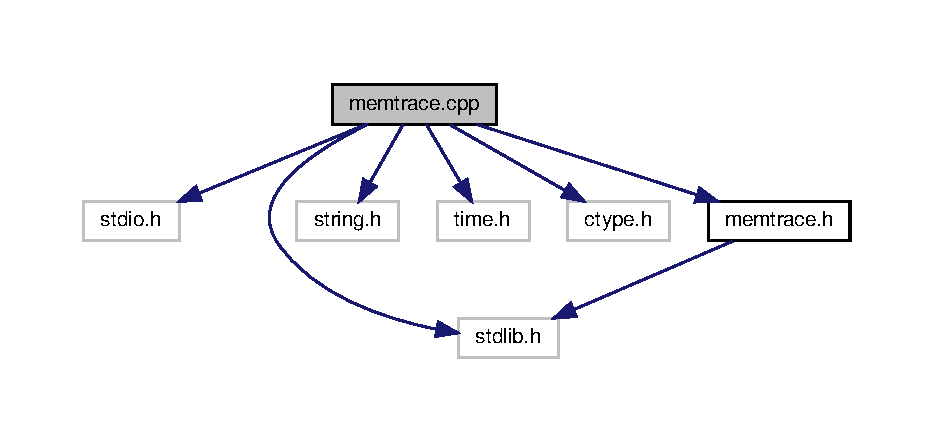
\includegraphics[width=350pt]{memtrace_8cpp__incl}
\end{center}
\end{figure}
\subsection*{Classes}
\begin{DoxyCompactItemize}
\item 
struct \textbf{ call\+\_\+t}
\item 
struct \textbf{ \+\_\+registry\+\_\+item}
\end{DoxyCompactItemize}
\subsection*{Macros}
\begin{DoxyCompactItemize}
\item 
\#define \textbf{ M\+E\+M\+T\+R\+A\+CE}
\item 
\#define \textbf{ F\+R\+O\+M\+\_\+\+M\+E\+M\+T\+R\+A\+C\+E\+\_\+\+C\+PP}
\item 
\#define \textbf{ F\+M\+A\+L\+L\+OC}~0
\item 
\#define \textbf{ F\+C\+A\+L\+L\+OC}~1
\item 
\#define \textbf{ F\+R\+E\+A\+L\+L\+OC}~2
\item 
\#define \textbf{ F\+F\+R\+EE}~3
\item 
\#define \textbf{ F\+N\+EW}~4
\item 
\#define \textbf{ F\+D\+E\+L\+E\+TE}~5
\item 
\#define \textbf{ F\+N\+E\+W\+A\+RR}~6
\item 
\#define \textbf{ F\+D\+E\+L\+E\+T\+E\+A\+RR}~7
\item 
\#define \textbf{ C\+O\+MP}(a,  d)~(((a)$<$=3 \&\& (d)$<$=3) $\vert$$\vert$ ((d)==(a)+1))
\item 
\#define \textbf{ PU}(p)~((char$\ast$)p+C\+A\+N\+A\+R\+Y\+\_\+\+L\+EN)
\item 
\#define \textbf{ P}(pu)~((char$\ast$)pu-\/C\+A\+N\+A\+R\+Y\+\_\+\+L\+EN)
\item 
\#define \textbf{ X\+S\+TR}(s)~\textbf{ S\+TR}(s)
\item 
\#define \textbf{ S\+TR}(s)~\#s
\end{DoxyCompactItemize}
\subsection*{Typedefs}
\begin{DoxyCompactItemize}
\item 
typedef \textbf{ E\+N\+D\+\_\+\+N\+A\+M\+E\+S\+P\+A\+CE} \textbf{ S\+T\+A\+R\+T\+\_\+\+N\+A\+M\+E\+S\+P\+A\+CE} struct \textbf{ \+\_\+registry\+\_\+item} \textbf{ registry\+\_\+item}
\end{DoxyCompactItemize}
\subsection*{Enumerations}
\begin{DoxyCompactItemize}
\item 
enum \textbf{ B\+O\+OL} \{ \textbf{ F\+A\+L\+SE}, 
\textbf{ T\+R\+UE}
 \}
\end{DoxyCompactItemize}
\subsection*{Functions}
\begin{DoxyCompactItemize}
\item 
void \textbf{ mem\+\_\+dump} (void const $\ast$mem, size\+\_\+t size, F\+I\+LE $\ast$fp)
\item 
int \textbf{ mem\+\_\+check} (void)
\item 
int \textbf{ allocated\+\_\+blocks} ()
\item 
\textbf{ E\+N\+D\+\_\+\+N\+A\+M\+E\+S\+P\+A\+CE} \textbf{ S\+T\+A\+R\+T\+\_\+\+N\+A\+M\+E\+S\+P\+A\+CE} void $\ast$ \textbf{ traced\+\_\+malloc} (size\+\_\+t size, const char $\ast$par\+\_\+txt, int line, const char $\ast$file)
\item 
void $\ast$ \textbf{ traced\+\_\+calloc} (size\+\_\+t count, size\+\_\+t size, const char $\ast$par\+\_\+txt, int line, const char $\ast$file)
\item 
void \textbf{ traced\+\_\+free} (void $\ast$pu, const char $\ast$par\+\_\+txt, int line, const char $\ast$file)
\item 
void $\ast$ \textbf{ traced\+\_\+realloc} (void $\ast$old, size\+\_\+t size, const char $\ast$par\+\_\+txt, int line, const char $\ast$file)
\end{DoxyCompactItemize}


\subsection{Macro Definition Documentation}
\mbox{\label{memtrace_8cpp_aaed1b7df4f99525f21eda754cf7fae05}} 
\index{memtrace.\+cpp@{memtrace.\+cpp}!C\+O\+MP@{C\+O\+MP}}
\index{C\+O\+MP@{C\+O\+MP}!memtrace.\+cpp@{memtrace.\+cpp}}
\subsubsection{C\+O\+MP}
{\footnotesize\ttfamily \#define C\+O\+MP(\begin{DoxyParamCaption}\item[{}]{a,  }\item[{}]{d }\end{DoxyParamCaption})~(((a)$<$=3 \&\& (d)$<$=3) $\vert$$\vert$ ((d)==(a)+1))}

\mbox{\label{memtrace_8cpp_af6fff8cbc37157865d4b383dacfd947b}} 
\index{memtrace.\+cpp@{memtrace.\+cpp}!F\+C\+A\+L\+L\+OC@{F\+C\+A\+L\+L\+OC}}
\index{F\+C\+A\+L\+L\+OC@{F\+C\+A\+L\+L\+OC}!memtrace.\+cpp@{memtrace.\+cpp}}
\subsubsection{F\+C\+A\+L\+L\+OC}
{\footnotesize\ttfamily \#define F\+C\+A\+L\+L\+OC~1}

\mbox{\label{memtrace_8cpp_a744b443f8bd1fad5895b111602c0ead9}} 
\index{memtrace.\+cpp@{memtrace.\+cpp}!F\+D\+E\+L\+E\+TE@{F\+D\+E\+L\+E\+TE}}
\index{F\+D\+E\+L\+E\+TE@{F\+D\+E\+L\+E\+TE}!memtrace.\+cpp@{memtrace.\+cpp}}
\subsubsection{F\+D\+E\+L\+E\+TE}
{\footnotesize\ttfamily \#define F\+D\+E\+L\+E\+TE~5}

\mbox{\label{memtrace_8cpp_acd2bfc6563a2ac0ae741ee31dfbf1c92}} 
\index{memtrace.\+cpp@{memtrace.\+cpp}!F\+D\+E\+L\+E\+T\+E\+A\+RR@{F\+D\+E\+L\+E\+T\+E\+A\+RR}}
\index{F\+D\+E\+L\+E\+T\+E\+A\+RR@{F\+D\+E\+L\+E\+T\+E\+A\+RR}!memtrace.\+cpp@{memtrace.\+cpp}}
\subsubsection{F\+D\+E\+L\+E\+T\+E\+A\+RR}
{\footnotesize\ttfamily \#define F\+D\+E\+L\+E\+T\+E\+A\+RR~7}

\mbox{\label{memtrace_8cpp_aa6b915326a446c2a67f05f5504d9bc30}} 
\index{memtrace.\+cpp@{memtrace.\+cpp}!F\+F\+R\+EE@{F\+F\+R\+EE}}
\index{F\+F\+R\+EE@{F\+F\+R\+EE}!memtrace.\+cpp@{memtrace.\+cpp}}
\subsubsection{F\+F\+R\+EE}
{\footnotesize\ttfamily \#define F\+F\+R\+EE~3}

\mbox{\label{memtrace_8cpp_a8817d7ba90cf2e1ddd83f35dbb862542}} 
\index{memtrace.\+cpp@{memtrace.\+cpp}!F\+M\+A\+L\+L\+OC@{F\+M\+A\+L\+L\+OC}}
\index{F\+M\+A\+L\+L\+OC@{F\+M\+A\+L\+L\+OC}!memtrace.\+cpp@{memtrace.\+cpp}}
\subsubsection{F\+M\+A\+L\+L\+OC}
{\footnotesize\ttfamily \#define F\+M\+A\+L\+L\+OC~0}

\mbox{\label{memtrace_8cpp_a9f98c384938a2ff256aa6a0a6f8992dc}} 
\index{memtrace.\+cpp@{memtrace.\+cpp}!F\+N\+EW@{F\+N\+EW}}
\index{F\+N\+EW@{F\+N\+EW}!memtrace.\+cpp@{memtrace.\+cpp}}
\subsubsection{F\+N\+EW}
{\footnotesize\ttfamily \#define F\+N\+EW~4}

\mbox{\label{memtrace_8cpp_afc0db05fd089296f53cc7e8441ebc565}} 
\index{memtrace.\+cpp@{memtrace.\+cpp}!F\+N\+E\+W\+A\+RR@{F\+N\+E\+W\+A\+RR}}
\index{F\+N\+E\+W\+A\+RR@{F\+N\+E\+W\+A\+RR}!memtrace.\+cpp@{memtrace.\+cpp}}
\subsubsection{F\+N\+E\+W\+A\+RR}
{\footnotesize\ttfamily \#define F\+N\+E\+W\+A\+RR~6}

\mbox{\label{memtrace_8cpp_afcc2cb9c3434359e629fdd446aab6175}} 
\index{memtrace.\+cpp@{memtrace.\+cpp}!F\+R\+E\+A\+L\+L\+OC@{F\+R\+E\+A\+L\+L\+OC}}
\index{F\+R\+E\+A\+L\+L\+OC@{F\+R\+E\+A\+L\+L\+OC}!memtrace.\+cpp@{memtrace.\+cpp}}
\subsubsection{F\+R\+E\+A\+L\+L\+OC}
{\footnotesize\ttfamily \#define F\+R\+E\+A\+L\+L\+OC~2}

\mbox{\label{memtrace_8cpp_ab4e504c96e3c59936ff0a9f31573b1b0}} 
\index{memtrace.\+cpp@{memtrace.\+cpp}!F\+R\+O\+M\+\_\+\+M\+E\+M\+T\+R\+A\+C\+E\+\_\+\+C\+PP@{F\+R\+O\+M\+\_\+\+M\+E\+M\+T\+R\+A\+C\+E\+\_\+\+C\+PP}}
\index{F\+R\+O\+M\+\_\+\+M\+E\+M\+T\+R\+A\+C\+E\+\_\+\+C\+PP@{F\+R\+O\+M\+\_\+\+M\+E\+M\+T\+R\+A\+C\+E\+\_\+\+C\+PP}!memtrace.\+cpp@{memtrace.\+cpp}}
\subsubsection{F\+R\+O\+M\+\_\+\+M\+E\+M\+T\+R\+A\+C\+E\+\_\+\+C\+PP}
{\footnotesize\ttfamily \#define F\+R\+O\+M\+\_\+\+M\+E\+M\+T\+R\+A\+C\+E\+\_\+\+C\+PP}

\mbox{\label{memtrace_8cpp_aa90f3e89fc3fe477370afb9f81975081}} 
\index{memtrace.\+cpp@{memtrace.\+cpp}!M\+E\+M\+T\+R\+A\+CE@{M\+E\+M\+T\+R\+A\+CE}}
\index{M\+E\+M\+T\+R\+A\+CE@{M\+E\+M\+T\+R\+A\+CE}!memtrace.\+cpp@{memtrace.\+cpp}}
\subsubsection{M\+E\+M\+T\+R\+A\+CE}
{\footnotesize\ttfamily \#define M\+E\+M\+T\+R\+A\+CE}

\mbox{\label{memtrace_8cpp_a64bc26cf9b35a1dabeb2a58a96bc9b99}} 
\index{memtrace.\+cpp@{memtrace.\+cpp}!P@{P}}
\index{P@{P}!memtrace.\+cpp@{memtrace.\+cpp}}
\subsubsection{P}
{\footnotesize\ttfamily \#define P(\begin{DoxyParamCaption}\item[{}]{pu }\end{DoxyParamCaption})~((char$\ast$)pu-\/C\+A\+N\+A\+R\+Y\+\_\+\+L\+EN)}

\mbox{\label{memtrace_8cpp_a5d3529a7e2c30650032e14a1dbc9aaac}} 
\index{memtrace.\+cpp@{memtrace.\+cpp}!PU@{PU}}
\index{PU@{PU}!memtrace.\+cpp@{memtrace.\+cpp}}
\subsubsection{PU}
{\footnotesize\ttfamily \#define PU(\begin{DoxyParamCaption}\item[{}]{p }\end{DoxyParamCaption})~((char$\ast$)p+C\+A\+N\+A\+R\+Y\+\_\+\+L\+EN)}

\mbox{\label{memtrace_8cpp_a6388870e639eee9c0a69446876f1f8cc}} 
\index{memtrace.\+cpp@{memtrace.\+cpp}!S\+TR@{S\+TR}}
\index{S\+TR@{S\+TR}!memtrace.\+cpp@{memtrace.\+cpp}}
\subsubsection{S\+TR}
{\footnotesize\ttfamily \#define S\+TR(\begin{DoxyParamCaption}\item[{}]{s }\end{DoxyParamCaption})~\#s}

\mbox{\label{memtrace_8cpp_a03943706e48069237cd57f2d35ca987e}} 
\index{memtrace.\+cpp@{memtrace.\+cpp}!X\+S\+TR@{X\+S\+TR}}
\index{X\+S\+TR@{X\+S\+TR}!memtrace.\+cpp@{memtrace.\+cpp}}
\subsubsection{X\+S\+TR}
{\footnotesize\ttfamily \#define X\+S\+TR(\begin{DoxyParamCaption}\item[{}]{s }\end{DoxyParamCaption})~\textbf{ S\+TR}(s)}



\subsection{Typedef Documentation}
\mbox{\label{memtrace_8cpp_a70b3f3b7e889e715810f67307625db45}} 
\index{memtrace.\+cpp@{memtrace.\+cpp}!registry\+\_\+item@{registry\+\_\+item}}
\index{registry\+\_\+item@{registry\+\_\+item}!memtrace.\+cpp@{memtrace.\+cpp}}
\subsubsection{registry\+\_\+item}
{\footnotesize\ttfamily typedef \textbf{ E\+N\+D\+\_\+\+N\+A\+M\+E\+S\+P\+A\+CE} \textbf{ S\+T\+A\+R\+T\+\_\+\+N\+A\+M\+E\+S\+P\+A\+CE} struct \textbf{ \+\_\+registry\+\_\+item}  \textbf{ registry\+\_\+item}}



\subsection{Enumeration Type Documentation}
\mbox{\label{memtrace_8cpp_a3e5b8192e7d9ffaf3542f1210aec18dd}} 
\index{memtrace.\+cpp@{memtrace.\+cpp}!B\+O\+OL@{B\+O\+OL}}
\index{B\+O\+OL@{B\+O\+OL}!memtrace.\+cpp@{memtrace.\+cpp}}
\subsubsection{B\+O\+OL}
{\footnotesize\ttfamily enum \textbf{ B\+O\+OL}}

\begin{DoxyEnumFields}{Enumerator}
\raisebox{\heightof{T}}[0pt][0pt]{\index{F\+A\+L\+SE@{F\+A\+L\+SE}!memtrace.\+cpp@{memtrace.\+cpp}}\index{memtrace.\+cpp@{memtrace.\+cpp}!F\+A\+L\+SE@{F\+A\+L\+SE}}}\mbox{\label{memtrace_8cpp_a3e5b8192e7d9ffaf3542f1210aec18ddaa1e095cc966dbecf6a0d8aad75348d1a}} 
F\+A\+L\+SE&\\
\hline

\raisebox{\heightof{T}}[0pt][0pt]{\index{T\+R\+UE@{T\+R\+UE}!memtrace.\+cpp@{memtrace.\+cpp}}\index{memtrace.\+cpp@{memtrace.\+cpp}!T\+R\+UE@{T\+R\+UE}}}\mbox{\label{memtrace_8cpp_a3e5b8192e7d9ffaf3542f1210aec18ddaa82764c3079aea4e60c80e45befbb839}} 
T\+R\+UE&\\
\hline

\end{DoxyEnumFields}


\subsection{Function Documentation}
\mbox{\label{memtrace_8cpp_a4ec27aa588e69e834e293374f5c14e67}} 
\index{memtrace.\+cpp@{memtrace.\+cpp}!allocated\+\_\+blocks@{allocated\+\_\+blocks}}
\index{allocated\+\_\+blocks@{allocated\+\_\+blocks}!memtrace.\+cpp@{memtrace.\+cpp}}
\subsubsection{allocated\+\_\+blocks()}
{\footnotesize\ttfamily int allocated\+\_\+blocks (\begin{DoxyParamCaption}{ }\end{DoxyParamCaption})}

\mbox{\label{memtrace_8cpp_ac6308f8e862dbc52b364a505483191a6}} 
\index{memtrace.\+cpp@{memtrace.\+cpp}!mem\+\_\+check@{mem\+\_\+check}}
\index{mem\+\_\+check@{mem\+\_\+check}!memtrace.\+cpp@{memtrace.\+cpp}}
\subsubsection{mem\+\_\+check()}
{\footnotesize\ttfamily int mem\+\_\+check (\begin{DoxyParamCaption}\item[{void}]{ }\end{DoxyParamCaption})}

\mbox{\label{memtrace_8cpp_a031b528c007e2e8ba5d814be13d3860c}} 
\index{memtrace.\+cpp@{memtrace.\+cpp}!mem\+\_\+dump@{mem\+\_\+dump}}
\index{mem\+\_\+dump@{mem\+\_\+dump}!memtrace.\+cpp@{memtrace.\+cpp}}
\subsubsection{mem\+\_\+dump()}
{\footnotesize\ttfamily void mem\+\_\+dump (\begin{DoxyParamCaption}\item[{void const $\ast$}]{mem,  }\item[{size\+\_\+t}]{size,  }\item[{F\+I\+LE $\ast$}]{fp }\end{DoxyParamCaption})}

\mbox{\label{memtrace_8cpp_a68998093ee624349c5cab1aab7bc915f}} 
\index{memtrace.\+cpp@{memtrace.\+cpp}!traced\+\_\+calloc@{traced\+\_\+calloc}}
\index{traced\+\_\+calloc@{traced\+\_\+calloc}!memtrace.\+cpp@{memtrace.\+cpp}}
\subsubsection{traced\+\_\+calloc()}
{\footnotesize\ttfamily void$\ast$ traced\+\_\+calloc (\begin{DoxyParamCaption}\item[{size\+\_\+t}]{count,  }\item[{size\+\_\+t}]{size,  }\item[{const char $\ast$}]{par\+\_\+txt,  }\item[{int}]{line,  }\item[{const char $\ast$}]{file }\end{DoxyParamCaption})}

\mbox{\label{memtrace_8cpp_a1f2006cf357ea01179f18a5c965ff105}} 
\index{memtrace.\+cpp@{memtrace.\+cpp}!traced\+\_\+free@{traced\+\_\+free}}
\index{traced\+\_\+free@{traced\+\_\+free}!memtrace.\+cpp@{memtrace.\+cpp}}
\subsubsection{traced\+\_\+free()}
{\footnotesize\ttfamily void traced\+\_\+free (\begin{DoxyParamCaption}\item[{void $\ast$}]{pu,  }\item[{const char $\ast$}]{par\+\_\+txt,  }\item[{int}]{line,  }\item[{const char $\ast$}]{file }\end{DoxyParamCaption})}

\mbox{\label{memtrace_8cpp_a30b6aa180e3214beb1f48c5a9381e5ac}} 
\index{memtrace.\+cpp@{memtrace.\+cpp}!traced\+\_\+malloc@{traced\+\_\+malloc}}
\index{traced\+\_\+malloc@{traced\+\_\+malloc}!memtrace.\+cpp@{memtrace.\+cpp}}
\subsubsection{traced\+\_\+malloc()}
{\footnotesize\ttfamily \textbf{ E\+N\+D\+\_\+\+N\+A\+M\+E\+S\+P\+A\+CE} \textbf{ S\+T\+A\+R\+T\+\_\+\+N\+A\+M\+E\+S\+P\+A\+CE} void$\ast$ traced\+\_\+malloc (\begin{DoxyParamCaption}\item[{size\+\_\+t}]{size,  }\item[{const char $\ast$}]{par\+\_\+txt,  }\item[{int}]{line,  }\item[{const char $\ast$}]{file }\end{DoxyParamCaption})}

\mbox{\label{memtrace_8cpp_aa9656d71bfbb848ef518892eb0e3909b}} 
\index{memtrace.\+cpp@{memtrace.\+cpp}!traced\+\_\+realloc@{traced\+\_\+realloc}}
\index{traced\+\_\+realloc@{traced\+\_\+realloc}!memtrace.\+cpp@{memtrace.\+cpp}}
\subsubsection{traced\+\_\+realloc()}
{\footnotesize\ttfamily void$\ast$ traced\+\_\+realloc (\begin{DoxyParamCaption}\item[{void $\ast$}]{old,  }\item[{size\+\_\+t}]{size,  }\item[{const char $\ast$}]{par\+\_\+txt,  }\item[{int}]{line,  }\item[{const char $\ast$}]{file }\end{DoxyParamCaption})}


\section{memtrace.\+h File Reference}
\label{memtrace_8h}\index{memtrace.\+h@{memtrace.\+h}}
{\ttfamily \#include $<$stdlib.\+h$>$}\newline
Include dependency graph for memtrace.\+h\+:
\nopagebreak
\begin{figure}[H]
\begin{center}
\leavevmode
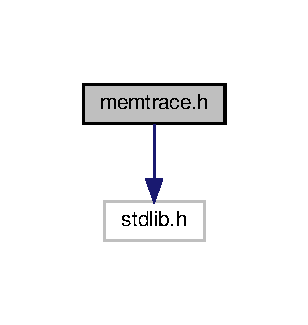
\includegraphics[width=148pt]{memtrace_8h__incl}
\end{center}
\end{figure}
This graph shows which files directly or indirectly include this file\+:
\nopagebreak
\begin{figure}[H]
\begin{center}
\leavevmode
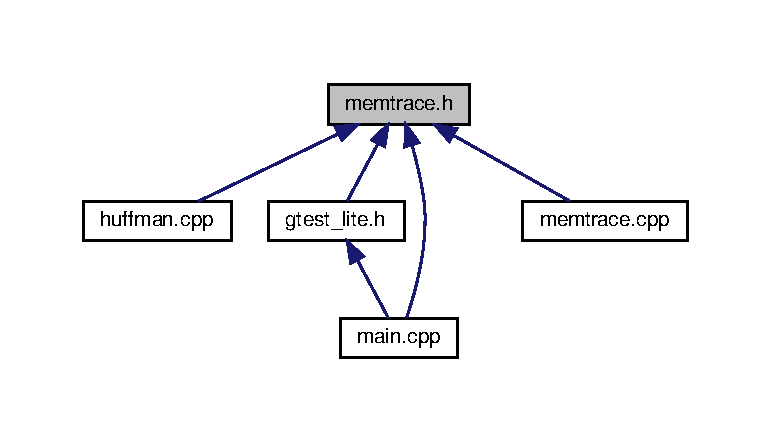
\includegraphics[width=350pt]{memtrace_8h__dep__incl}
\end{center}
\end{figure}
\subsection*{Macros}
\begin{DoxyCompactItemize}
\item 
\#define \textbf{ M\+E\+M\+T\+R\+A\+CE}
\item 
\#define \textbf{ M\+E\+M\+T\+R\+A\+C\+E\+\_\+\+T\+O\+\_\+\+M\+E\+M\+O\+RY}
\item 
\#define \textbf{ M\+E\+M\+T\+R\+A\+C\+E\+\_\+\+A\+U\+TO}
\item 
\#define \textbf{ M\+E\+M\+T\+R\+A\+C\+E\+\_\+C}
\item 
\#define \textbf{ A\+L\+L\+O\+W\+\_\+\+F\+R\+E\+E\+\_\+\+N\+U\+LL}
\item 
\#define \textbf{ S\+T\+A\+R\+T\+\_\+\+N\+A\+M\+E\+S\+P\+A\+CE}
\item 
\#define \textbf{ E\+N\+D\+\_\+\+N\+A\+M\+E\+S\+P\+A\+CE}
\item 
\#define \textbf{ T\+R\+A\+C\+EC}(func)~func
\item 
\#define \textbf{ T\+H\+R\+O\+W\+\_\+\+B\+A\+D\+A\+L\+L\+OC}~throw (std\+::bad\+\_\+alloc)
\item 
\#define \textbf{ T\+H\+R\+O\+W\+\_\+\+N\+O\+T\+H\+I\+NG}~throw ()
\item 
\#define \textbf{ malloc}(size)~\textbf{ T\+R\+A\+C\+EC}(\textbf{ traced\+\_\+malloc})(size,\#size,\+\_\+\+\_\+\+L\+I\+N\+E\+\_\+\+\_\+,\+\_\+\+\_\+\+F\+I\+L\+E\+\_\+\+\_\+)
\item 
\#define \textbf{ calloc}(count,  size)~\textbf{ T\+R\+A\+C\+EC}(\textbf{ traced\+\_\+calloc})(count, size, \#count\char`\"{},\char`\"{}\#size,\+\_\+\+\_\+\+L\+I\+N\+E\+\_\+\+\_\+,\+\_\+\+\_\+\+F\+I\+L\+E\+\_\+\+\_\+)
\item 
\#define \textbf{ free}(p)~\textbf{ T\+R\+A\+C\+EC}(\textbf{ traced\+\_\+free})(p, \#p,\+\_\+\+\_\+\+L\+I\+N\+E\+\_\+\+\_\+,\+\_\+\+\_\+\+F\+I\+L\+E\+\_\+\+\_\+)
\item 
\#define \textbf{ realloc}(old,  size)~\textbf{ T\+R\+A\+C\+EC}(\textbf{ traced\+\_\+realloc})(old,size,\#size,\+\_\+\+\_\+\+L\+I\+N\+E\+\_\+\+\_\+,\+\_\+\+\_\+\+F\+I\+L\+E\+\_\+\+\_\+)
\end{DoxyCompactItemize}
\subsection*{Functions}
\begin{DoxyCompactItemize}
\item 
\textbf{ S\+T\+A\+R\+T\+\_\+\+N\+A\+M\+E\+S\+P\+A\+CE} int \textbf{ allocated\+\_\+blocks} ()
\item 
\textbf{ E\+N\+D\+\_\+\+N\+A\+M\+E\+S\+P\+A\+CE} \textbf{ S\+T\+A\+R\+T\+\_\+\+N\+A\+M\+E\+S\+P\+A\+CE} int \textbf{ mem\+\_\+check} (void)
\item 
void $\ast$ \textbf{ traced\+\_\+malloc} (size\+\_\+t size, const char $\ast$size\+\_\+txt, int line, const char $\ast$file)
\item 
void $\ast$ \textbf{ traced\+\_\+calloc} (size\+\_\+t count, size\+\_\+t size, const char $\ast$size\+\_\+txt, int line, const char $\ast$file)
\item 
void \textbf{ traced\+\_\+free} (void $\ast$p, const char $\ast$size\+\_\+txt, int line, const char $\ast$file)
\item 
void $\ast$ \textbf{ traced\+\_\+realloc} (void $\ast$old, size\+\_\+t size, const char $\ast$size\+\_\+txt, int line, const char $\ast$file)
\item 
void \textbf{ mem\+\_\+dump} (void const $\ast$mem, size\+\_\+t size, F\+I\+LE $\ast$fp)
\end{DoxyCompactItemize}


\subsection{Macro Definition Documentation}
\mbox{\label{memtrace_8h_af30a73f26c0085429afe8d13ccf255f5}} 
\index{memtrace.\+h@{memtrace.\+h}!A\+L\+L\+O\+W\+\_\+\+F\+R\+E\+E\+\_\+\+N\+U\+LL@{A\+L\+L\+O\+W\+\_\+\+F\+R\+E\+E\+\_\+\+N\+U\+LL}}
\index{A\+L\+L\+O\+W\+\_\+\+F\+R\+E\+E\+\_\+\+N\+U\+LL@{A\+L\+L\+O\+W\+\_\+\+F\+R\+E\+E\+\_\+\+N\+U\+LL}!memtrace.\+h@{memtrace.\+h}}
\subsubsection{A\+L\+L\+O\+W\+\_\+\+F\+R\+E\+E\+\_\+\+N\+U\+LL}
{\footnotesize\ttfamily \#define A\+L\+L\+O\+W\+\_\+\+F\+R\+E\+E\+\_\+\+N\+U\+LL}

\mbox{\label{memtrace_8h_ab98a612296b79e3e44d41727977b07a5}} 
\index{memtrace.\+h@{memtrace.\+h}!calloc@{calloc}}
\index{calloc@{calloc}!memtrace.\+h@{memtrace.\+h}}
\subsubsection{calloc}
{\footnotesize\ttfamily \#define calloc(\begin{DoxyParamCaption}\item[{}]{count,  }\item[{}]{size }\end{DoxyParamCaption})~\textbf{ T\+R\+A\+C\+EC}(\textbf{ traced\+\_\+calloc})(count, size, \#count\char`\"{},\char`\"{}\#size,\+\_\+\+\_\+\+L\+I\+N\+E\+\_\+\+\_\+,\+\_\+\+\_\+\+F\+I\+L\+E\+\_\+\+\_\+)}

\mbox{\label{memtrace_8h_a28886d59fbdc2dccd82cc4887e967d0d}} 
\index{memtrace.\+h@{memtrace.\+h}!E\+N\+D\+\_\+\+N\+A\+M\+E\+S\+P\+A\+CE@{E\+N\+D\+\_\+\+N\+A\+M\+E\+S\+P\+A\+CE}}
\index{E\+N\+D\+\_\+\+N\+A\+M\+E\+S\+P\+A\+CE@{E\+N\+D\+\_\+\+N\+A\+M\+E\+S\+P\+A\+CE}!memtrace.\+h@{memtrace.\+h}}
\subsubsection{E\+N\+D\+\_\+\+N\+A\+M\+E\+S\+P\+A\+CE}
{\footnotesize\ttfamily \#define E\+N\+D\+\_\+\+N\+A\+M\+E\+S\+P\+A\+CE}

\mbox{\label{memtrace_8h_a9d4b5df3530d1bc733070a4669ba6ebc}} 
\index{memtrace.\+h@{memtrace.\+h}!free@{free}}
\index{free@{free}!memtrace.\+h@{memtrace.\+h}}
\subsubsection{free}
{\footnotesize\ttfamily \#define free(\begin{DoxyParamCaption}\item[{}]{p }\end{DoxyParamCaption})~\textbf{ T\+R\+A\+C\+EC}(\textbf{ traced\+\_\+free})(p, \#p,\+\_\+\+\_\+\+L\+I\+N\+E\+\_\+\+\_\+,\+\_\+\+\_\+\+F\+I\+L\+E\+\_\+\+\_\+)}

\mbox{\label{memtrace_8h_a2eb0b03d1a9de9615a291b1205969069}} 
\index{memtrace.\+h@{memtrace.\+h}!malloc@{malloc}}
\index{malloc@{malloc}!memtrace.\+h@{memtrace.\+h}}
\subsubsection{malloc}
{\footnotesize\ttfamily \#define malloc(\begin{DoxyParamCaption}\item[{}]{size }\end{DoxyParamCaption})~\textbf{ T\+R\+A\+C\+EC}(\textbf{ traced\+\_\+malloc})(size,\#size,\+\_\+\+\_\+\+L\+I\+N\+E\+\_\+\+\_\+,\+\_\+\+\_\+\+F\+I\+L\+E\+\_\+\+\_\+)}

\mbox{\label{memtrace_8h_aa90f3e89fc3fe477370afb9f81975081}} 
\index{memtrace.\+h@{memtrace.\+h}!M\+E\+M\+T\+R\+A\+CE@{M\+E\+M\+T\+R\+A\+CE}}
\index{M\+E\+M\+T\+R\+A\+CE@{M\+E\+M\+T\+R\+A\+CE}!memtrace.\+h@{memtrace.\+h}}
\subsubsection{M\+E\+M\+T\+R\+A\+CE}
{\footnotesize\ttfamily \#define M\+E\+M\+T\+R\+A\+CE}

\mbox{\label{memtrace_8h_ac7d83b17b55e7ca775a0127988f45c30}} 
\index{memtrace.\+h@{memtrace.\+h}!M\+E\+M\+T\+R\+A\+C\+E\+\_\+\+A\+U\+TO@{M\+E\+M\+T\+R\+A\+C\+E\+\_\+\+A\+U\+TO}}
\index{M\+E\+M\+T\+R\+A\+C\+E\+\_\+\+A\+U\+TO@{M\+E\+M\+T\+R\+A\+C\+E\+\_\+\+A\+U\+TO}!memtrace.\+h@{memtrace.\+h}}
\subsubsection{M\+E\+M\+T\+R\+A\+C\+E\+\_\+\+A\+U\+TO}
{\footnotesize\ttfamily \#define M\+E\+M\+T\+R\+A\+C\+E\+\_\+\+A\+U\+TO}

\mbox{\label{memtrace_8h_abd343745021a44232eb2808e547001d5}} 
\index{memtrace.\+h@{memtrace.\+h}!M\+E\+M\+T\+R\+A\+C\+E\+\_\+C@{M\+E\+M\+T\+R\+A\+C\+E\+\_\+C}}
\index{M\+E\+M\+T\+R\+A\+C\+E\+\_\+C@{M\+E\+M\+T\+R\+A\+C\+E\+\_\+C}!memtrace.\+h@{memtrace.\+h}}
\subsubsection{M\+E\+M\+T\+R\+A\+C\+E\+\_\+C}
{\footnotesize\ttfamily \#define M\+E\+M\+T\+R\+A\+C\+E\+\_\+C}

\mbox{\label{memtrace_8h_ac089c2c8a58531c78e528190c18946b0}} 
\index{memtrace.\+h@{memtrace.\+h}!M\+E\+M\+T\+R\+A\+C\+E\+\_\+\+T\+O\+\_\+\+M\+E\+M\+O\+RY@{M\+E\+M\+T\+R\+A\+C\+E\+\_\+\+T\+O\+\_\+\+M\+E\+M\+O\+RY}}
\index{M\+E\+M\+T\+R\+A\+C\+E\+\_\+\+T\+O\+\_\+\+M\+E\+M\+O\+RY@{M\+E\+M\+T\+R\+A\+C\+E\+\_\+\+T\+O\+\_\+\+M\+E\+M\+O\+RY}!memtrace.\+h@{memtrace.\+h}}
\subsubsection{M\+E\+M\+T\+R\+A\+C\+E\+\_\+\+T\+O\+\_\+\+M\+E\+M\+O\+RY}
{\footnotesize\ttfamily \#define M\+E\+M\+T\+R\+A\+C\+E\+\_\+\+T\+O\+\_\+\+M\+E\+M\+O\+RY}

\mbox{\label{memtrace_8h_a2d566601d9a416502dd2fd2816678fed}} 
\index{memtrace.\+h@{memtrace.\+h}!realloc@{realloc}}
\index{realloc@{realloc}!memtrace.\+h@{memtrace.\+h}}
\subsubsection{realloc}
{\footnotesize\ttfamily \#define realloc(\begin{DoxyParamCaption}\item[{}]{old,  }\item[{}]{size }\end{DoxyParamCaption})~\textbf{ T\+R\+A\+C\+EC}(\textbf{ traced\+\_\+realloc})(old,size,\#size,\+\_\+\+\_\+\+L\+I\+N\+E\+\_\+\+\_\+,\+\_\+\+\_\+\+F\+I\+L\+E\+\_\+\+\_\+)}

\mbox{\label{memtrace_8h_aad4cd792b953244f20869915267ae837}} 
\index{memtrace.\+h@{memtrace.\+h}!S\+T\+A\+R\+T\+\_\+\+N\+A\+M\+E\+S\+P\+A\+CE@{S\+T\+A\+R\+T\+\_\+\+N\+A\+M\+E\+S\+P\+A\+CE}}
\index{S\+T\+A\+R\+T\+\_\+\+N\+A\+M\+E\+S\+P\+A\+CE@{S\+T\+A\+R\+T\+\_\+\+N\+A\+M\+E\+S\+P\+A\+CE}!memtrace.\+h@{memtrace.\+h}}
\subsubsection{S\+T\+A\+R\+T\+\_\+\+N\+A\+M\+E\+S\+P\+A\+CE}
{\footnotesize\ttfamily \#define S\+T\+A\+R\+T\+\_\+\+N\+A\+M\+E\+S\+P\+A\+CE}

\mbox{\label{memtrace_8h_ad51e1559346aea8b3493be2ecefaa09d}} 
\index{memtrace.\+h@{memtrace.\+h}!T\+H\+R\+O\+W\+\_\+\+B\+A\+D\+A\+L\+L\+OC@{T\+H\+R\+O\+W\+\_\+\+B\+A\+D\+A\+L\+L\+OC}}
\index{T\+H\+R\+O\+W\+\_\+\+B\+A\+D\+A\+L\+L\+OC@{T\+H\+R\+O\+W\+\_\+\+B\+A\+D\+A\+L\+L\+OC}!memtrace.\+h@{memtrace.\+h}}
\subsubsection{T\+H\+R\+O\+W\+\_\+\+B\+A\+D\+A\+L\+L\+OC}
{\footnotesize\ttfamily \#define T\+H\+R\+O\+W\+\_\+\+B\+A\+D\+A\+L\+L\+OC~throw (std\+::bad\+\_\+alloc)}

\mbox{\label{memtrace_8h_ab62d0ac94900b7586e89da2d6cedf008}} 
\index{memtrace.\+h@{memtrace.\+h}!T\+H\+R\+O\+W\+\_\+\+N\+O\+T\+H\+I\+NG@{T\+H\+R\+O\+W\+\_\+\+N\+O\+T\+H\+I\+NG}}
\index{T\+H\+R\+O\+W\+\_\+\+N\+O\+T\+H\+I\+NG@{T\+H\+R\+O\+W\+\_\+\+N\+O\+T\+H\+I\+NG}!memtrace.\+h@{memtrace.\+h}}
\subsubsection{T\+H\+R\+O\+W\+\_\+\+N\+O\+T\+H\+I\+NG}
{\footnotesize\ttfamily \#define T\+H\+R\+O\+W\+\_\+\+N\+O\+T\+H\+I\+NG~throw ()}

\mbox{\label{memtrace_8h_a429dce7f3bb9a1335f0c7febd62938df}} 
\index{memtrace.\+h@{memtrace.\+h}!T\+R\+A\+C\+EC@{T\+R\+A\+C\+EC}}
\index{T\+R\+A\+C\+EC@{T\+R\+A\+C\+EC}!memtrace.\+h@{memtrace.\+h}}
\subsubsection{T\+R\+A\+C\+EC}
{\footnotesize\ttfamily \#define T\+R\+A\+C\+EC(\begin{DoxyParamCaption}\item[{}]{func }\end{DoxyParamCaption})~func}



\subsection{Function Documentation}
\mbox{\label{memtrace_8h_ab8ef9a94a4ba8246012e9bfeb5b0c589}} 
\index{memtrace.\+h@{memtrace.\+h}!allocated\+\_\+blocks@{allocated\+\_\+blocks}}
\index{allocated\+\_\+blocks@{allocated\+\_\+blocks}!memtrace.\+h@{memtrace.\+h}}
\subsubsection{allocated\+\_\+blocks()}
{\footnotesize\ttfamily \textbf{ S\+T\+A\+R\+T\+\_\+\+N\+A\+M\+E\+S\+P\+A\+CE} int allocated\+\_\+blocks (\begin{DoxyParamCaption}{ }\end{DoxyParamCaption})}

\mbox{\label{memtrace_8h_ab531f5bcfca2f50b8c2a43f7bb96fc0e}} 
\index{memtrace.\+h@{memtrace.\+h}!mem\+\_\+check@{mem\+\_\+check}}
\index{mem\+\_\+check@{mem\+\_\+check}!memtrace.\+h@{memtrace.\+h}}
\subsubsection{mem\+\_\+check()}
{\footnotesize\ttfamily \textbf{ E\+N\+D\+\_\+\+N\+A\+M\+E\+S\+P\+A\+CE} \textbf{ S\+T\+A\+R\+T\+\_\+\+N\+A\+M\+E\+S\+P\+A\+CE} int mem\+\_\+check (\begin{DoxyParamCaption}\item[{void}]{ }\end{DoxyParamCaption})}

\mbox{\label{memtrace_8h_a031b528c007e2e8ba5d814be13d3860c}} 
\index{memtrace.\+h@{memtrace.\+h}!mem\+\_\+dump@{mem\+\_\+dump}}
\index{mem\+\_\+dump@{mem\+\_\+dump}!memtrace.\+h@{memtrace.\+h}}
\subsubsection{mem\+\_\+dump()}
{\footnotesize\ttfamily void mem\+\_\+dump (\begin{DoxyParamCaption}\item[{void const $\ast$}]{mem,  }\item[{size\+\_\+t}]{size,  }\item[{F\+I\+LE $\ast$}]{fp }\end{DoxyParamCaption})}

\mbox{\label{memtrace_8h_a8d30ad82fb5ab2f070bb8552d5f71575}} 
\index{memtrace.\+h@{memtrace.\+h}!traced\+\_\+calloc@{traced\+\_\+calloc}}
\index{traced\+\_\+calloc@{traced\+\_\+calloc}!memtrace.\+h@{memtrace.\+h}}
\subsubsection{traced\+\_\+calloc()}
{\footnotesize\ttfamily void$\ast$ traced\+\_\+calloc (\begin{DoxyParamCaption}\item[{size\+\_\+t}]{count,  }\item[{size\+\_\+t}]{size,  }\item[{const char $\ast$}]{size\+\_\+txt,  }\item[{int}]{line,  }\item[{const char $\ast$}]{file }\end{DoxyParamCaption})}

\mbox{\label{memtrace_8h_a324b3ee7c799b67c4bae9dcdfa144dd3}} 
\index{memtrace.\+h@{memtrace.\+h}!traced\+\_\+free@{traced\+\_\+free}}
\index{traced\+\_\+free@{traced\+\_\+free}!memtrace.\+h@{memtrace.\+h}}
\subsubsection{traced\+\_\+free()}
{\footnotesize\ttfamily void traced\+\_\+free (\begin{DoxyParamCaption}\item[{void $\ast$}]{p,  }\item[{const char $\ast$}]{size\+\_\+txt,  }\item[{int}]{line,  }\item[{const char $\ast$}]{file }\end{DoxyParamCaption})}

\mbox{\label{memtrace_8h_a878d95f35f94bc40ca0f41d5630c10a0}} 
\index{memtrace.\+h@{memtrace.\+h}!traced\+\_\+malloc@{traced\+\_\+malloc}}
\index{traced\+\_\+malloc@{traced\+\_\+malloc}!memtrace.\+h@{memtrace.\+h}}
\subsubsection{traced\+\_\+malloc()}
{\footnotesize\ttfamily void$\ast$ traced\+\_\+malloc (\begin{DoxyParamCaption}\item[{size\+\_\+t}]{size,  }\item[{const char $\ast$}]{size\+\_\+txt,  }\item[{int}]{line,  }\item[{const char $\ast$}]{file }\end{DoxyParamCaption})}

\mbox{\label{memtrace_8h_ad9b9f054074d56c2952702d341aba982}} 
\index{memtrace.\+h@{memtrace.\+h}!traced\+\_\+realloc@{traced\+\_\+realloc}}
\index{traced\+\_\+realloc@{traced\+\_\+realloc}!memtrace.\+h@{memtrace.\+h}}
\subsubsection{traced\+\_\+realloc()}
{\footnotesize\ttfamily void$\ast$ traced\+\_\+realloc (\begin{DoxyParamCaption}\item[{void $\ast$}]{old,  }\item[{size\+\_\+t}]{size,  }\item[{const char $\ast$}]{size\+\_\+txt,  }\item[{int}]{line,  }\item[{const char $\ast$}]{file }\end{DoxyParamCaption})}


\hypertarget{node_8cpp}{}\section{node.\+cpp File Reference}
\label{node_8cpp}\index{node.\+cpp@{node.\+cpp}}
{\ttfamily \#include \char`\"{}node.\+h\char`\"{}}\newline

\hypertarget{node_8h}{}\section{node.\+h File Reference}
\label{node_8h}\index{node.\+h@{node.\+h}}
{\ttfamily \#include \char`\"{}letter.\+h\char`\"{}}\newline
{\ttfamily \#include $<$cstdlib$>$}\newline
\subsection*{Classes}
\begin{DoxyCompactItemize}
\item 
class \hyperlink{class_node}{Node}
\item 
class \hyperlink{class_end}{End}
\item 
class \hyperlink{class_path}{Path}
\end{DoxyCompactItemize}

%--- End generated contents ---

% Index
\backmatter
\newpage
\phantomsection
\clearemptydoublepage
\addcontentsline{toc}{chapter}{Index}
\printindex

\end{document}
